




%\section[Transportation Governance Modeling][Gouvernance du Système de Transport]{Transportation Governance Modeling}{Modélisation de la Gouvernance du Système de Transport} 
\section{Co-evolution and governance}{Co-évolution et gouvernance} 


\label{sec:lutecia}


%----------------------------------------------------------------------------------------


%\bpar{
%This part makes a step further towards more complex models. A toy-model introducing governance processes is described. Such exploration logically enters our theoretical framework to try to validate the network necessity assumption : if non-linear necessary processes are highlighted and validated against stylized facts, it argues towards the validation of this assumption. 
%}{
%Cette section fait un pas supplémentaire vers des modèles plus complexes. Un modèle jouet incluant des processus de gouvernance est décrit. Cette exploration répond de manière logique à notre cadre théorique et aux études précédentes, en particulier pour essayer de valider l'hypothèse de nécessité des réseaux : si des processus non-linéaires sont montrés nécessaires pour la validation sur des faits stylisés, cela pousse à argumenter pour sa validité.
%}


\bpar{
This section aims at giving directions for a more complex modeling of co-evolution, still at the mesoscopic scale. We have seen in~\ref{sec:networkterritories} that governance processes correspond to a level that intrinsically couples networks and territories: collective decisions concern jointly transportation, territories, and their articulation. We have moreover studied the particular case of a Mega-city Region (MCR) in~\ref{sec:casestudies}, and saw to what extent this context favoured a complexity of interactions. The emergence of MCR raises the question of the emergence of new governance modes, more or less easy to implement as show the examples of Stuttgart and the Rhin-Rhur matropolitan areas according to~\cite{lenechet2017peupler}.
}{
Cette section se propose de donner des pistes vers une modélisation plus complexe de la co-évolution, toujours à l'échelle mesoscopique. Nous avons vu en~\ref{sec:networkterritories} que les processus de gouvernance relevaient d'un niveau qui couple intrinsèquement les réseaux et les territoires : les décisions collectives portent à la fois sur les transports, les territoires et leur articulation. Nous avons par ailleurs étudié le cas particulier d'une méga-région urbaine (MCR) en~\ref{sec:casestudies}, et vu dans quelle mesure ce contexte était propice à une complexité des interactions. L'émergence des MCR soulève la question de l'émergence de nouveaux modes de gouvernance, plus ou moins aisés à mettre en place comme en témoignent selon~\cite{lenechet2017peupler} les exemples de la métropole de Stuttgart et de la métropole Rhin-Rhur.
}


\bpar{
We develop therefore here a co-evolution model at the scale of a MCR, which aims in particular at endogenizing some processes of governance of the transportation network. This model extends in particular the one introduced by~\cite{le2010approche} which was then developed by~\cite{lenechet:halshs-00674059}.
}{
Nous développons donc ici un modèle de co-évolution à l'échelle d'une MCR, qui vise en particulier à endogénéiser certains processus de gouvernance du réseau de transport. Ce modèle étend en particulier celui introduit par~\cite{le2010approche} puis développé par~\cite{lenechet:halshs-00674059}.
}





%----------------------------------------------------------------------------------------


%%%%%%%%%%%%%%%%%%%%
\subsection{Context}{Contexte}


\subsubsection{Mega-city regions and Gouvernance}{Mega-régions urbaines et gouvernance}


\bpar{
We recall that a mega-city region is a network of highly connected cities in terms of economic and population flows, forming a polycentric region~\cite{hall2006polycentric}. It is the last ``urban regime'' which emerged within systems of cities, and it could be a more plausible trajectory for large urban agglomerates than always larger monocentric cities. \cite{neuman2009futures} point out that the future sustainability of these MCR will be closely linked to their ability to \emph{learn} new governance schemes, in the sense of an increased adaptability and flexibility of governance processes. \cite{innes2010strategies} suggest also that strategies implying self-organisation through the dialogue between stakeholders is a path to tackle the complexity of governing a MCR. We propose in the following to partly answer this question of the link between governance structure and evolution of the MCR, through the model we will develop.
}{
Nous rappelons qu'une méga-région urbaine est un réseau de villes fortement connecté en termes de flux économiques et de population, formant une région polycentrique~\cite{hall2006polycentric}. Il s'agit du dernier ``régime urbain'' qui a émergé au sein des systèmes de villes, et il pourrait s'agir d'une trajectoire plus plausible que des villes monocentriques toujours plus grandes pour les agglomérats urbains considérables. \cite{neuman2009futures} soulignent que la soutenabilité future de ces MCR sera intimement liée à leur capacité à \emph{apprendre} de nouveaux schémas de gouvernance, au sens d'une adaptabilité et flexibilité accrue des processus de gouvernance. \cite{innes2010strategies} suggèrent par ailleurs que des stratégies impliquant auto-organisation par le dialogue entre acteurs sont un moyen de répondre efficacement à la complexité de la gouvernance d'une MCR. Nous proposons par la suite de répondre partiellement à cette question du lien entre structure de gouvernance et évolution de la MCR, par l'intermédiaire du modèle que nous développons. 
}



\subsubsection{Modeling co-evolution with governance processes}{Modélisation de la co-évolution par des processus de gouvernance}


\bpar{
The role of governance processes in models coupling the evolution of transportation network with the evolution of land-use has already been investigated from different points of view in modeling approaches.
}{
Le rôle des processus de gouvernance dans les modèles couplant l'évolution des réseaux de transport à l'évolution de l'usage du sol a déjà été considéré selon différents points de vue dans les approches de modélisation.
}

\paragraph{Network growth}{Croissance du réseau}

\bpar{
\cite{li2016integrated} couples a network investment model with a traffic and localization model, and show that the obtained steady state configurations outperform an operational research approach to network design in terms of overall accessibility.
}{
\cite{li2016integrated} couple un modèle d'investissement de réseau avec un modèle de traffic et de localisation, et montre que les solutions stationnaires obtenues sont plus performantes qu'une approche en recherche opérationnelle pour la conception du réseau en termes d'accessibilité totale.
}

\bpar{
Concerning network growth only, \cite{jacobs2016transport} proposes a simulation model in which alternatives between plausible investments (by different investors) are evaluated with a discrete choice model which utility function takes into account returns on investment but also variables to optimize such as accessibility. It is applied to the growth of the Dutch railway in the 19th century, and shown to reproduce quite accurately the historical network.
}{
Concernant la croissance du réseau seule, \cite{jacobs2016transport} propose un modèle de simulation dans lequel les alternatives entre investissements plausibles (par des investisseurs différents) sont évalués avec un modèle de choix discrets dont la fonction d'utilité prend en compte les retours sur investissement mais également des variables à optimiser comme l'accessibilité. Il est appliqué à la croissance du réseau ferré néerlandais au 19ème siècle, et démontré capable de reproduire assez fidèlement le réseau historique. 
}


\paragraph{Modeling gouvernance}{Modéliser la gouvernance}

\bpar{
\cite{Xie2011} introduces a theoretical economic model of infrastructure investment. Two levels of governance, local and centralized are considered in the model. For the provision of new infrastructure that has to be split between two contiguous districts (space being one-dimensional), a game between governance agents determines both the level of decision and the attribution of the stock proportion to each district. Governments either want to maximize the aggregated utility (Pigovian government), or include explicit political strategies to satisfy a median voter. Numerical exploration of the model show that these processes are equivalent to compromises between cost and benefits, and that the level of governance depends on the state of the network.
}{
\cite{Xie2011} introduit un modèle économique théorique d'investissement dans les infrastructures. Deux niveaux de gouvernance, local et centralisé, sont considérés dans le modèle. Pour la provision d'une nouvelle infrastructure qui doit être partagée entre deux zones contiguës (l'espace étant à une dimension), un jeu entre des agents de gouvernance détermine à la fois le niveau de décision et l'attribution de proportion du stock à chaque zone. Les gouvernements veulent soit maximiser l'utilité agrégée (gouvernement Pigovien), ou bien inclure des stratégies politiques explicites pour satisfaire un électeur médian. L'exploration numérique du modèle montre que ces processus sont équivalents à des compromis entre coûts et bénéfices, et que le niveau de gouvernance effectif dépend de l'état du réseau.
}

\bpar{
\cite{xie2011governance} proposes a more simple version of this model on the governance side but coupled with a more realistic travel side : it couples on a synthetic growing network a traffic model with a pricing model and an investment model, and show that under the assumption of centralization, an equilibrium between demand and network performance can be reached, but that investments are not efficient on the long run, with a higher loss for decentralized investments.
}{
\cite{xie2011governance} propose une version plus simple de ce modèle du point de vue de la gouvernance mais couplé à un modèle de transport plus réaliste : il couple sur un réseau synthétique croissant un modèle de traffic avec un modèle de prix et un modèle d'investissement, et montre que sous l'hypothèse d'une centralisation, un équilibre entre la demande et la performance du réseau peut être atteint, mais que les investissements ne sont pas efficients sur le long terme, avec une perte plus importante pour les investissements décentralisés.
}

\bpar{
We will be positioned in a logic close to the first model for the role of the governance structure, and close to the second for the precision of the inclusion of space.
}{
Nous nous placerons dans une logique proche du premier modèle dans le rôle de la structure de gouvernance, et proche du second dans la précision de prise en compte de l'espace.
}

\paragraph{Game theory}{Théorie des jeux}

\bpar{
Some of these models, in particular \cite{Xie2011}, are based on game theory to model the behavior of stakeholders. It has already been widely applied for modeling in social and political sciences to questions dealing with cognitive interacting agents with individual interests~\cite{ordeshook1986game}. \cite{abler1977spatial} (p.~487) formulate a location decision problem for coffee farms on Kilimanjaro as a game combining a production strategy and a location strategy (fixing then the environmental conditions). This framework has furthermore already been used in transportation investment studies, such as e.g. in~\cite{Roumboutsos2008209} which use the notion of Nash equilibrium to understand choices of public or private operators concerning the integration of their system in the broader mobility system. We will use game theory paradigms to integrate governance in a simple way in our model.
}{
Certains de ces modèles, en particulier \cite{Xie2011}, se fondent sur la théorie des jeux pour modéliser le comportement des acteurs. Celle-ci a déjà été largement appliquée à des questions de modélisation en sciences sociales ou politiques pour des problèmes impliquant des agents cognitifs en interaction avec des intérêts individuels~\cite{ordeshook1986game}. \cite{abler1977spatial} (p.~487) formulent un problème de décision de localisation pour des fermes de café au Kilimanjaro comme un jeu combinant une stratégie de production et une stratégie de localisation (fixant alors les conditions environnementales). Ce cadre a par ailleurs été utilisé pour étudier les investissements en termes de transports, comme par exemple par \cite{Roumboutsos2008209} qui utilisent la notion d'équilibre de Nash pour comprendre les choix des opérateurs publics ou privés quant à l'intégration de leur système dans le système de mobilité plus global. Nous utiliserons des paradigmes de théorie des jeux pour intégrer la gouvernance de manière simple dans notre modèle.
}


%\subsubsection{Objective}{Objectif}


\bpar{
The aim of this section is thus to follow these different models, and to propose a co-evolution model in which network growth is integrated in an endogenous way, through the modeling of implied governance processes.
}{
Le but de cette section est donc de se placer dans la lignée de ces différents modèles, et de proposer un modèle de co-évolution au sein duquel la croissance du réseau est intégrée de manière endogène, par la modélisation des processus de gouvernance impliqués.
}




%%%%%%%%%%%%%%%%%%%%
\subsection{The Lutecia Model}{Le Modèle Lutecia}


\bpar{
We now describe the Lutecia model\footnote{The name comes from an acronym linked to its structure which is detailed in the following. Naming models is a delicate operation since it induces a kind of reification or even personification, in any case can be seen as a kind of fetichism. It can potentially perturb the role of the model within the knowledge production process and make the model an end in itself. We are convinced that an endogenous naming through the uses of the model by the community is more appropriate. We make here an exception given the particular story of its genesis.}, in its general structure, and then in the specification we will later develop.
}{
Nous décrivons à présent le modèle Lutecia\footnote{L'appellation est un acronyme lié à sa structure détaillée par la suite. Nommer les modèles est une opération délicate puisqu'elle induit une certaine réification voire personification, dans tous les cas relève d'un certain fétichisme. Celle-ci peut potentiellement perturber la place du modèle au sein du processus de production de connaissance et faire du modèle une fin en soi. Nous sommes convaincu qu'une dénomination endogène via les usages du modèles par la communauté est plus approprié. Nous faisons ici une exception vu l'histoire particulière de sa genèse.}, dans sa structure générale, puis dans la spécification que nous développerons par la suite.
}


\subsubsection{Global model structure}{Structure globale du modèle}


\bpar{
The model couples in a complex way a module for land-use evolution with a module for transportation network growth. Submodels (or submodules), detailed in the following, include in particular a governance module that rules processes of network evolution. The most important feature of the Lutecia model is the inclusion of an endogenous infrastructure provision submodel, based on iterative increases in accessibility, within a Luti model.
}{
Le modèle couple de manière complexe un module pour l'évolution de l'usage du sol à un module de croissance de réseau de transport. Les sous-modèles (ou modules), détaillés par la suite, incluent en particulier un modèle de gouvernance pour régir l'évolution du réseau. L'inclusion d'un modèle endogène de provision d'infrastructures basé sur les augmentation itératives de l'accessibilité, au sein d'un modèle Luti, consiste en la contribution principale du modèle Lutecia.
}

\bpar{
The accessibility, that we will take here as a potential of access of actives to employments, is a cornerstone of the model. Indeed, micro-economic agents will relocate in order to maximize their accessibility, whereas new transportation infrastructure decisions will be taken by governance agents based on a criteria of maximization of accessibility increase in their area.
}{
L'accessibilité, que nous prendrons ici comme un potentiel d'accès des actifs aux emplois, est au coeur du modèle. En effet, les agents micro-économiques se relocalisent afin de maximiser leur accessibilité, tandis que les décisions de nouvelles infrastructures de transport sont prises par des agents de gouvernance selon un critère de maximisation de l'augmentation d'accessibilité dans leur zone. 
}

\bpar{
In its more general structure, the Lutecia model is composed by five sub-models, of which only three will be studied here for simplicity reasons. The sub-models are the following :
\begin{itemize}
\item LU stands for Land Use module : it proceeds to the re-localization of actives and employments given current conditions of accessibility.
\item T stands for Transport module : it computes the transportation conditions such as flows and congestion in the urban region.
\item EC stands for Evaluation of Cooperation module : it evaluates the agent or agents that will proceed to build a new infrastructure. 
\item I stands for Infrastructure provision module : it determines the localization of the new transportation infrastructure, based on a criteria of accessibility maximization.
\item A stands for Agglomeration economies module : it evaluates the productivity of firms, depending on the accessibility to employments.
\end{itemize}
We will in the following study the coupling between the LU-EC-I sub-models: we assume at the first order no significant effect of congestion, and thus no role of transport modeling; and furthermore consider simple assumptions for economics and neglect agglomeration economies.
}{
Dans sa structure la plus générale, le modèle Lutecia est composé de cinq sous-modèles, parmi lesquels nous n'en développerons que trois ici pour des raisons de simplicité. Les sous-modèles sont les suivants :
\begin{itemize}
	\item LU correspond à l'usage du sol : il opère la relocalisation des actifs et des emplois étant donné les conditions courantes d'accessibilité.
	\item T correspond à Transport : il évalue les conditions de transport (flux, congestion) dans la région urbaine.
	\item EC correspond à l'évaluation de la coopération : il évalue le ou les agents qui procéderont à la construction d'une nouvelle infrastructure.
	\item I correspond à provision d'infrastructure : il détermine la localisation de la nouvelle infrastructure de transport en fonction d'un critère de maximisation d'accessibilité.
	\item A correspond aux agglomérations d'économie : il évalue la productivité des firmes, selon l'accessibilité aux emplois.
\end{itemize}
Nous étudierons par la suite le couplage entre les sous-modèles LU-EC-I : nous supposons au premier ordre pas d'effet significatif de la congestion, et donc pas de rôle de la modélisation du transport ; et par ailleurs prenons des hypothèses simples sur le plan économique et négligeons les agglomérations d'économie.
}


\bpar{
Different time scales are included in the model: a short scale, corresponding to daily mobility that yields flows in the transportation network and to firms productivity (modules T and A); an intermediate scale for residential and firms dynamics (module LU) ; and a long time scale for the evolution of the network (modules EC and I). Levels of stochasticity are considered accordingly: the smallest scales have deterministic dynamics whereas the longer exhibits randomness.
}{
Des échelles de temps imbriquées sont incluses dans le modèle : une échelle courte, correspondant à la mobilité quotidienne qui produit les flux dans le réseau de transport et aux productivités des entreprises (modules T et A) ; une échelle intermédiaire pour les dynamiques de localisation des actifs et emplois (module LU) ; et une longue échelle de temps pour l'évolution du réseau (modules EC et I). Les niveau de stochasticité sont pris en conséquence : les échelles les plus petites ont des dynamiques déterministes tandis que la plus longue présente un comportement aléatoire.
}


\subsubsection{Detailed description of the model}{Description détaillée du modèle}

\paragraph{Description of the environment}{Description de l'environnement}


\bpar{
The mega-city region is modeled with a two level spatial zoning. The world is composed by a lattice of patches, that are the basic units to quantify land use. We assume that each patch $k$ is characterized at time $t$ by its resident actives $A_k(t)$ and number of employments $E_k(t)$. At a higher level, the MCR is decomposed into administrative areas that correspond to the city governance levels, to which we attribute $M$ abstract agents called \emph{mayors}: $M_k$ gives thus the administrative area to which each patch belongs. We assume furthermore the existence of a global governance agent that correspond to a regional authority at the level of the MCR.
}{
La méga-région Urbaine est modélisée avec un zonage spatial à deux niveaux. L'environnement du modèle est composé par une grille, dont les cellules sont les unités élémentaires pour quantifier l'usage du sol. Nous supposons que chaque cellule $k$ est caractérisée au temps $t$ par le nombre d'actifs y résidant $A_k(t)$ et son nombre d'emplois $E_k(t)$. À un niveau supérieur, la MCR est décomposée en unités administratives qui correspondent au niveau de gouvernance des villes, auxquelles sont attribués $M$ agents abstraits appelés \emph{maires} : $M_k$ désigne ainsi la zone administrative à laquelle chaque cellule appartient. Nous supposons de plus l'existence d'un agent de gouvernance global qui correspond à une autorité typiquement régionale, au niveau de la MCR.
}

\bpar{
On top of this patch-level land-use and governance setup, we introduce a transportation network $G = (V,E)$ localized in space by its nodes coordinates $(x_v,y_v)$, and characterized by a speed $v_G$ relative to movements in the euclidian space. Assuming that the network can be taken anywhere on each link, it unequivocally induces a geographical travel-time distance that we describe by the shortest path distance matrix between each patch $D = (d_{k,k'}(t))$. The accessibility of actives to employments is then defined for each patch as a Hansen accessibility with a decay of distance $\lambda$ capturing typical commuting range, by
}{
De manière complémentaire à cette configuration d'usage du sol et de gouvernance, nous introduisons un réseau de transport $G = (V,E)$ localisé dans l'espace par les coordonnées de ses noeuds $(x_v,y_v)$, et caractérisé par une vitesse $v_G$ relative aux déplacements dans l'espace euclidien. Sous l'hypothèse que le réseau peut être rejoint à tout endroit sur les liens, il induit de manière univoque une distance-temps géographique, que nous décrivons par la matrice des plus courts temps entre chaque cellule $D = (d_{k,k'}(t))$. L'accessibilité des actifs aux emplois est alors définie pour chaque cellule comme une accessibilité de Hansen, avec un paramètre de décroissance de la distance $\lambda$ qui capture un potentiel d'accès des actifs aux emplois, par
}


\begin{equation}
X^{(A)}_k = A_k\cdot \sum_{k'} E_{k'} \exp{\left(-\lambda \cdot d_{k,k'}\right)}
\end{equation}


\bpar{
The accessibility of employments to actives is defined in a similar manner. Dynamics are taken in a discrete way: $t \in \{t_0 = 0 , \ldots , t_f\}$, with time ticks corresponding to a time scale at which land use typically evolves, i.e. 5 to 10 years. We take thus a slower speed for the evolution of the network which will be constructed by segments at each time step, whereas land-use will be considered as being in equilibrium at the scale of the decade, in consistence with the frame developed in chapter~\ref{ch:thematic}.
}{
L'accessibilité des emplois aux actifs est définie de manière similaire. La dynamique est considérée de façon discrete : $t \in \{t_0 = 0 , \ldots , t_f\}$, avec les pas de temps correspondant à une échelle à laquelle l'usage du sol évolue en moyenne, i.e. de 5 à 10 ans. Nous prenons ainsi une vitesse plus lente pour l'évolution du réseau qui se construira par tronçons à chaque pas de temps, tandis que l'usage du sol sera considéré comme en équilibre à l'échelle de la décade, en cohérence avec le cadre développé en chapitre~\ref{ch:thematic}.
}



%%%%%%
%%% - not useful

%\subsubsection{NW  - JR Protocole de décision de construction infra : cas un seul acteur}{}

%Given a single actor and an already budgeted infrastructure, we make an intermediate assumption of rationality of planning. More precisely, the actor seeks to optimize the accessibility gain for all its patches. 


\paragraph{Evolution of land-use}{Évolution de l'usage du sol}


\bpar{
For the land-use module, the model is based on the Lowry model~\cite{lowry1964model}. We assume that residential/employments relocations are at equilibrium at the time scale of a tick. In comparison, the evolution of transportation infrastructure is much slower~\citep{wegener2004land}\footnote{We do not consider land values, rents or transportation costs, that are the core of models in Urban Economics such as the Alonso and Fujita models for example (see \cite{lemoy2017exploring} for a recent agent-based approach to these).}. Actives and Employments relocate given some utilities that take into account both accessibility and the urban form. Indeed, one of the drivers of Urban Sprawl may be interpreted as a repulsion of residents by density. To aggregate both effects in a simple way, we take a Cobb-douglas function for utilities of actives and employments
}{
Pour le module d'usage du sol, le modèle s'inspire du modèle de Lowry~\cite{lowry1964model}. Les relocalisations d'une proportion fixe d'actifs et d'emplois sont supposées à l'équilibre à l'échelle d'un pas de temps. En comparaison, l'évolution de l'infrastructure de transport est largement plus lente~\cite{wegener2004land}\footnote{Nous ne considérons pas ici les valeurs foncières, les loyers ou les coûts de transport, qui sont au coeur des modèles d'économie urbaine comme le modèle d'Alonso ou de Fujita par exemple (voir \cite{lemoy2017exploring} pour une approche récente multi-agents de ceux-ci).}. Les actifs et les emplois se relocalisent selon des utilités qui prennent en compte à la fois l'accessibilité et la forme urbaine. En effet, l'un des moteurs de l'étalement urbain peut être interprété comme une répulsion des résidents par la densité. Pour agréger les deux effets, nous prenons une fonction de Cobb-Douglas pour l'utilité
}

\begin{equation}\label{eq:utility}
U_k^{(A)} = {X_k^{(A)}}^{\gamma_A}\cdot {F_k^{(A)}}^{1-\gamma_A}
\end{equation}
%\[
%U_j (E) = X_j(E)^{\gamma_E}\cdot {F_j(E)}^{1-\gamma_E} ; F_j(E) = 1
%\]

\bpar{
what is equivalent to have a linear aggregation of the logarithm of explicative variables. Employments follow an analog expression with a dedicated weight parameter $\gamma_E$. Here the utility is simply influenced only by accessibility and by an indicator of local urban form called \emph{form factor}, given in the case of actives by $F_k^{(A)} = \frac{1}{A_k \cdot E_k}$, meaning that population is repulsed by density. The combination of the positive effect of accessibility to the negative effect of density produces a tension between contradictory objectives allowing a certain level of complexity already in the land-use sub-model alone. The form factor for jobs is taken as $F_k^{(E)}=1$ for the sake of simplicity and following the fact that jobs can aggregate far more than dwellings. 
}{
ce qui est équivalent à une agrégation linéaire du logarithme des variables explicatives. Les emplois suivent une expression analogue avec un paramètre de poids spécifique $\gamma_E$. L'utilité est influencée ici uniquement par l'accessibilité et par un indicateur de forme urbaine locale nommé \emph{facteur de forme}. Nous le définissons dans le cas des actifs par $F_k^{(A)} = \frac{1}{A_k \cdot E_k}$, ce qui signifie que la population est repoussée par la densité. La combinaison de l'effet positif de l'accessibilité à celui négatif de la densité produit une tension entre des objectifs contradictoires, permettant un certain niveau de complexité déjà dans le sous-modèle d'usage du sol seul. Le facteur de forme pour les emplois est pris comme $F_k^{(E)}=1$ pour simplifier et suivant la logique que les emplois peuvent s'agréger bien plus que les logements.
}

\bpar{
Relocations are then done deterministically following a discrete choice model, which yields the value of actives at the next step as
}{
Les relocalisations sont ensuite faites de manière déterministe suivant un modèle de choix discret, qui donne les valeurs des actifs à l'étape suivante comme
}

\begin{equation}\label{eq:discretechoicereloc}
A_i(t+1) = \alpha \cdot \sum_i{A_i(t)}\cdot\frac{\exp{(\beta U_i(A))}}{\sum_i{\exp{(\beta U_i(A))}}}
\end{equation}
%\[
%E_j(t+1) = \sum_j{E_j(t)}\cdot\frac{\exp{(\beta U_j(E))}}{\sum_j{\exp{(\beta U_j(E))}}}
%\]

\bpar{
where $\beta$ is the Discrete Choice parameter that can be interpreted as a ``level of randomness''\footnote{When $\beta \rightarrow 0$, all destination patches have an equal probability from any origin patch, whereas $\beta \rightarrow \infty$ gives fully deterministic behavior towards the patch with the best utility.}. $\alpha$ is the fixed fraction of actives relocating. Employments follow again a similar expression.
}{
où $\beta$ est le paramètre de choix discrets qui peut être interprété comme un ``niveau d'aléatoire''\footnote{Quand $\beta \rightarrow 0$, toutes les cellules de destination ont une probabilité égale depuis l'ensemble des cellules d'origine, tandis que $\beta \rightarrow \infty$ donne un comportement totalement déterministe vers la cellule avec meilleure utilité.}. $\alpha$ est la fraction fixe d'actif se relocalisant. Les emplois suivent une expression similaire.
}




\subsubsection{Network evolution : governance process}{Évolution du réseau : processus de gouvernance}



\paragraph{Assumptions}{Hypothèses}

\bpar{
The governance part of the model has the following rationale :
\begin{itemize}
\item Three levels of governance are included, namely a central actor (the region, or regional government), local actors (municipalities) acting individually, and local actors cooperating what constitutes an intermediate level.
\item Assuming a new infrastructure is to be built, the planning can be either from top-down decision (region) or from the bottom-up (local actors). We make the assumption that the processes behind the determination of the level of decision are far too complex (since they are generally political processes) to be taken into account in the model. This step is thus determined exogenously following an uniform law given a parameter.
\item If the decision is taken at the local level, negotiations between actors occur. We assume that
\begin{itemize}
\item the initiator of the new infrastructure can be any of the local actors, but richer cities will have more chance to built;
\item negotiations for possible collaboration are only done between neighbor cities, what is related to the medium range of infrastructure segments considered;
\item for this reason, and as $n$-players games have been shown to exhibit a chaotic behavior~\cite{2016arXiv161208111S} when $n$ increases, we consider negotiations between two actors only. The probability of cooperation that are endogenously determined can be furthermore directly interpreted.
\end{itemize}
\item For the sake of simplicity, the total stock of infrastructure built at one governance time step is constant, and decision times are also fixed\footnote{See the discussion for the implications of that hypothesis and possible relaxations.}.
\end{itemize}
}{
Le sous-modèle pour la gouvernance suit les hypothèses suivantes.
\begin{itemize}
	\item Trois niveaux de gouvernance sont inclus, qui sont un acteur central (la région, ou le gouvernement régional), les acteurs locaux (municipalités) qui agissent seuls, et les acteurs locaux qui coopèrent.%, ce qui constitue un niveau abstrait intermédiaire.%\comment{faire un schema ici}
	\item Sous l'hypothèse qu'une nouvelle infrastructure doit être construite, la planification peut être soit par le haut (région) soit par le bas (acteurs locaux). Nous supposons que les processus derrière la détermination du niveau de décision sont bien trop complexes (puisqu'il incluent généralement des processus politiques) pour être pris en compte par le modèle. Cette étape est donc déterminée de manière exogène selon une loi uniforme à paramètre fixe.%\footnote{Une piste alternative pour endogénéiser ce processus est proposée dans les développements.}.
	\item Si la décision est prise au niveau local, des négociations entre les acteurs ont lieu. Les concernant, nous supposons que :
	\begin{itemize}
		\item l'initiateur de la nouvelle infrastructure peut être n'importe quel acteur local, mais les villes riches ont plus de chance de construire ;
		\item les négociations pour des possibles collaborations n'ont lieu qu'entre acteurs voisins, ce qui est en cohérence avec des segments d'infrastructure de longueur moyenne ;
		\item pour cette raison, et d'autant plus que les jeux à $n$ joueurs présentent des comportements chaotiques quand $n$ augmente~\cite{2016arXiv161208111S}, nous ne considérons des négociations qu'entre deux acteurs uniquement. De plus, la probabilité de coopération endogène peut alors être directement interprétée.
	\end{itemize}
	\item Pour rester simple, le stock total d'infrastructure construit à un pas de temps de gouvernance est constant, et les temps de décision sont également fixés\footnote{Voir également la discussion pour de possibles relaxations de ces hypothèses.}.
\end{itemize}
}





%\comment[JR]{justify our simplistic choice of maximizing accessibility ; \cite{levinson2012forecasting} investigate far more precise rules of network growth but no interacting actors nor co-evolution, and more based on transportation constraints. In a similar vein, \cite{xie2009jurisdictional} compares centralized vs decentralized network growth, what is close to some questions we are tackling}

%\cite{yusufzyanova2011forecasting} very similar structure with global and local.


\paragraph{Network evolution}{Évolution du réseau}

\bpar{
The workflow for transportation network development is the following :
\begin{enumerate}
\item At each time step, 2 new road segments of length $l_r$ are built. The choice between local and global is done by a uniform draw with probability $\xi$. In the case of local building, roads are attributed successively to mayors (one road maximum per mayor) with probabilities $\xi_i$ which are proportional to the number of employments of each, what means that richer areas will get more roads.
\item Areas building a road will enter negotiations. Possible strategies for players (negotiating areas, $i=0,1$, the strategies being written $S_i$) are to not collaborate ($NC$), i.e. develop his road segment alone, and to collaborate ($C$), i.e. wanting to develop conjointly. Strategies are chosen simultaneously (non-cooperative game), in a random way according probabilities determined as detailed below. For $(C,NC)$ and $(NC,C)$ combinations, roads are built separately. For $(NC,NC)$ both act as alone, and for $(C,C)$ a common development is done.
\item Depending on the level of governance and the strategies chosen, the corresponding optimal infrastructures are build.
\end{enumerate}
}{
Les étapes pour le développement du réseau de transport sont les suivantes.
\begin{enumerate}
	\item À chaque pas de temps, 2 nouveaux segments de route de longueur $l_r$ sont construits. Le choix entre le niveau local et global est déterminé par un tirage uniforme avec une probabilité $\xi$. Dans le cas d'une construction locale, les routes sont attribuées successivement aux maires (une route par maire au maximum) avec des probabilités $\xi_i$ qui sont proportionnelles au nombre d'emplois de chacun, ce qui signifie que les zones plus riches auront plus de routes.
	\item Les zones devant construire chacune une route entrent en négociations. Les stratégies possibles pour les acteurs (zones en négociation, $i=0,1$, les stratégies étant notées $S_i$) sont de ne pas collaborer ($NC$), c'est-à-dire développer son tronçon de réseau seul, et de collaborer ($C$), c'est-à-dire vouloir développer conjointement. Les stratégies sont choisies simultanément (jeu non-coopératif), de manière aléatoire selon des probabilités déterminées comme détaillé ci-dessous. Pour les combinaisons $(C,NC)$ et $(NC,C)$, les routes sont construites séparément. Pour $(NC,NC)$ les deux agissent séparément et pour $(C,C)$ un développement commun est mené.
	\item Selon le niveau de gouvernance et les stratégies choisies, l'infrastructure optimale correspondante est construite.
\end{enumerate}
}


\paragraph{Evaluation of cooperation}{Évaluation de la coopération}

\bpar{
We detail now the way the cooperation probabilities are established. We denote $Z^{\ast}_i(S_0,S_1)$ the optimal infrastructure for area $i$ with $(S_0,S_1)\in \{(NC,C),(C,NC),(NC,NC)\}$ which are determined by an heuristic in each zone separately (see implementation details), and $Z^{\ast}_C$ the optimal common infrastructure computed with a 2 segments infrastructure on the union of both areas. It corresponds to the case where both strategies are $C$. Marginal accessibilities for area $i$ and infrastructure $Z$ is defined as $\Delta X_i(Z)=X^Z_i - X_i$. We introduce construction costs, noted $I$ for a road segment, assumed spatially uniform. We furthermore introduce a cost of collaboration $J$ that corresponds to a shared cost for building a larger infrastructure.
}{
Détaillons à présent la manière dont les probabilités de coopération sont établies. Nous notons $Z^{\ast}_i(S_0,S_1)$ l'infrastructure optimale en termes de gain d'accessibilité pour la zone $i$ avec $(S_0,S_1)\in \{(NC,C),(C,NC),(NC,NC)\}$ qui sont déterminées de manière heuristique pour chaque zone séparément (voir détails d'implémentation), et $Z^{\ast}_C$ l'infrastructure optimale commune calculée sur l'union des deux zones avec une infrastructure composée de deux segments élémentaires. Cette dernière correspond au cas où les deux stratégies sont $C$. Les accessibilités marginales pour la zone $i$ et l'infrastructure $Z$ sont définies comme $\Delta X_i(Z)=X^Z_i - X_i$. Nous introduisons des coûts de construction, notés $I$ pour un segment de route, supposés uniformes dans l'espace. Nous introduisons de plus un coût de collaboration $J$ qui correspond à un coût partagé pour construire une infrastructure plus grande.
}



\bpar{
The determination of probabilities defining mixed strategies is based on the payoff matrix, which gives is the value of utility gains for each players and each possible decision configuration. The payoff matrix of the game is the following, with $\kappa$ a normalization constant (``price of accessibility''), and the players being written $i\in \{ 0;1\}$ (such that $1-i$ denotes the player opposed to $i$)
}{
La détermination des probabilités donnant la composition des stratégies mixtes se base sur la matrice de gain, qui donne les gains d'utilité pour chaque joueur et chaque combinaison de décisions. La matrice de gain du jeu est la suivante, avec $\kappa$ une constante de normalisation (``prix de l'accessibilité''), et les joueurs étant notés $i\in \{ 0;1\}$ (tel que $1-i$ désigne le joueur opposé à $i$)
}

\begin{center}
\begin{tabular}{ |c|c|c| } 
 \hline
 0 $|$ 1  & C & NC \\ \hline
 C & $U_i = \kappa \cdot \Delta X_i(Z^{\ast}_C) - I - \frac{J}{2}$
   & $\begin{cases}U_0 = \kappa \cdot \Delta X_0(Z^{\ast}_0)-I \\U_1 = \kappa \cdot \Delta X_1(Z^{\ast}_1)-I - \frac{J}{2}\end{cases}$ \\ \hline
 NC & $\begin{cases}U_0 = \kappa \cdot \Delta X_0(Z^{\ast}_0)-I - \frac{J}{2}\\U_1 = \kappa \cdot \Delta X_1(Z^{\ast}_1)-I\end{cases}$
   & $U_i = \kappa \cdot \Delta X_i(Z^{\ast}_i) - I$ \\
 \hline
\end{tabular}
\end{center}


\bpar{
To simplify, we assume the cost parameters dimensioned as an accessibility what is equivalent to have $\kappa = 1$. We will furthermore see that since only accessibility differentials are determining, the construction cost $I$ does finally not play any role. This payoff matrix is used in two games corresponding to complementary processes:
\begin{itemize}
	\item the coordination game in which players have a mixed strategy, and for which we consider the Nash equilibrium\footnote{A Nash equilibrium is a strategy point in a discrete non-collaborative game for which no player can improve his gain by changing his strategy~\cite{ordeshook1986game}.} for corresponding probabilities, which implies a competition between players;
	\item an heuristic according to which players take their decision following a discrete choice model. It implies only a maximization of the utility gain and an indirect competition only.
\end{itemize}
}{
Pour simplifier, nous supposerons les paramètres de coût redimensionnés à une accessibilité ce qui revient à avoir $\kappa = 1$. Nous verrons par ailleurs que seuls des différentiels d'utilité étant déterminants, le coût de construction $I$ ne joue finalement pas de rôle. Cette matrice de gain est utilisée dans deux jeux traduisant des processus complémentaires :
\begin{itemize}
	\item le jeu de coordination dans lequel les joueurs ont une stratégie mixte, et pour lequel nous considérons l'équilibre de Nash\footnote{Un équilibre de Nash est un point de stratégies dans un jeu discret non-collaboratif pour lequel aucun joueur ne peut améliorer son gain en changeant sa stratégie~\cite{ordeshook1986game}.} pour les probabilités correspondantes, qui implique une compétition entre les joueurs ;
	\item une heuristique selon laquelle les joueurs prennent leur décision suivant un modèle de choix discrets. Celle-ci implique uniquement une maximisation du gain d'utilité et une compétition indirecte seulement.
\end{itemize}
}

\bpar{
We write $p_i = \Pb{S_i = C}$ the probability of each player to collaborate.
}{
Notons $p_i = \Pb{S_i = C}$ la probabilité de chaque joueur de collaborer.
}


\paragraph{Nash equilibrium}{Equilibre de Nash}

\bpar{
We can solve the mixed strategy Nash Equilibrium for this coordination game in all generality. We detail the computation in Appendix~\ref{app:sec:lutecia}. By writing $U_i(S_i,S_{1-i})$ the full payoff matrix, we have the expression of probabilities
}{
L'équilibre de Nash à stratégie mixte pour ce jeu non-coopératif peut être obtenu en toute généralité. Nous détaillons le calcul en Annexe~\ref{app:sec:lutecia}. En écrivant $U_i(S_i,S_{1-i})$ la matrice de gain complète, on a l'expression des probabilités
}

\[
p_{1-i} = - \frac{U_i(C,NC) - U_i(NC,NC)}{\left(U_i(C,C) - U_i(NC,C)\right) - \left(U_i(C,NC) - U_i(NC,NC)\right)}
\]

\bpar{
What gives with the expression of utilities previously given,
}{
Ce qui donne avec les expressions des utilités données précédemment,
}

\begin{equation}
p_i = \frac{J}{\Delta X_{1 - i}{Z^{\star}_{C}} - \Delta X_{1 - i}{Z^{\star}_{1 - i}}}
\end{equation}


\bpar{
This expression can be interpreted the following way: in this competitive game, the likelihood of a player to cooperate will decrease as the other player gain increases, and somehow counterintuitively, will increase as collaboration cost increases. The realism of this assumption must thus be moderated, and we can assume that in practice the equilibrium is never reached.
}{
Cette expression peut être interprétée de la façon suivante : dans ce jeu compétitif, la chance qu'un joueur coopère décroit quand le gain de l'autre joueur augmente, et d'une certaine manière contre-intuitif, s'accroit quand le coût de collaboration augmente. Le réalisme de cette hypothèse est donc à modérer, et nous pouvons supposer que l'équilibre n'est en pratique jamais atteint.
}

\bpar{
It also forces feasibility conditions on $J$ and accessibility gains to keep a probability. These are
\begin{itemize}
	\item $ J \leq \Delta X_{1 - i}(Z^{\star}_{C}) - \Delta X_{1 - i}(Z^{\star}_{1 - i})$, what can be interpreted as a cost-benefits condition, i.e. that the gain induced by the common infrastructure must be larger than the collaboration cost;
	\item $\Delta X_{1 - i}(Z^{\star}_{C}) \leq \Delta X_{1 - i}(Z^{\star}_{1 - i})$, i.e. that the gain induced by the common infrastructure must be positive.
\end{itemize}
}{
Cela impose également des conditions de faisabilité pour $J$ et les gains d'accessibilité pour conserver une probabilité. Celles-ci sont :
\begin{itemize}
	\item $ J \leq \Delta X_{1 - i}(Z^{\star}_{C}) - \Delta X_{1 - i}(Z^{\star}_{1 - i})$, qui s'interprète comme une condition coût-bénéfices, c'est-à-dire que le gain induit par l'infrastructure commune doit être supérieur au coût de collaboration ;
	\item $\Delta X_{1 - i}(Z^{\star}_{C}) \leq \Delta X_{1 - i}(Z^{\star}_{1 - i})$, c'est-à-dire que le gain induit par l'infrastructure commune doit être positif.
\end{itemize}
}




\paragraph{Discrete choice decisions}{Décisions par choix discrets}


\bpar{
Using the same utility functions, a random utility model for a discrete choice allows also to obtain expressions for probabilities. We have for player $i$ the utility differential between the choice $C$ and the choice $NC$ given by
}{
Avec les mêmes fonctions d'utilité, un modèle d'utilité aléatoire pour un choix discret permet également d'obtenir des expressions des probabilités. On a pour le joueur $i$ le différentiel d'utilité entre le choix $C$ et le choix $NC$ donné par
}

\[
U_i(C) - U_i(NC) = p_{1 - i} \left( \Delta X_{i}{Z^{\star}_{C}} - \Delta X_{i}{Z^{\star}_{i}}\right) - J
\]


\bpar{
Under the classical assumption of a model with a random utility distributed following a Gumbel law~\cite{ben1985discrete}, we have $\Pb{S_i=C} = \frac{1}{1 + \exp{[-\beta_{DC}(U_i(C) - U_i(NC))]}}$, where $\beta_{DC}$ is the discrete choice parameter (that we will fix at a large value $\beta_{DC} = 400$, by supposing a certain determinism at this level, since there is then a second random level).
}{
Sous l'hypothèse classique d'un modèle d'utilité aléatoire distribuée en loi de Gumbel~\cite{ben1985discrete}, on a $\Pb{S_i=C} = \frac{1}{1 + \exp{[-\beta_{DC}(U_i(C) - U_i(NC))]}}$, où $\beta_{DC}$ est le paramètre de choix discrets (que nous fixerons grand $\beta_{DC} = 400$, en supposant un certain déterminisme à ce niveau, puisqu'on a ensuite un deuxième niveau aléatoire). 
}


\bpar{
We substitute the expression of $p_{i-1}$ in the expression of $p_i$, what leads $p_i$ to verify the following equation
}{
On substitue l'expression de $p_{1-i}$ dans l'expression de $p_i$, ce qui conduit $p_i$ à vérifier l'équation suivante
}

\begin{equation}
p_i = \frac{1}{1 + \exp{\left(-\beta_{DC}\cdot \left(\frac{\Delta X_{i}{Z^{\star}_{C}} - \Delta X_{i}{Z^{\star}_{i}}}{1 + \exp{\left(- \beta_{DC}(p_i \cdot (\Delta X_{1 - i}(Z^{\star}_{C}) - \Delta X_{\bar{i}}(Z^{\star}_{1 - i})) - J)\right)}} - J \right)\right)}}
\end{equation}


\bpar{
We demonstrate (see Appendix~\ref{app:sec:lutecia}) that there always exists a solution $p_i \in [0,1]$, and we solve it numerically in the model to determine the probability to cooperate.
}{
Nous démontrons (voir Annexe~\ref{app:sec:lutecia}) qu'il existe toujours une solution $p_i \in [0,1]$, et nous la résolvons numériquement dans le modèle pour déterminer la probabilité de collaboration.
}


\paragraph{Random decision}{Décision aléatoire}


\bpar{
We also consider a reference mechanism, which does not assume negotiations, but which in the case of a local decision draws randomly a mayor, following an uniform law with probabilities proportional to the number of employments of each.
}{
Nous considérons également un mécanisme de référence, qui ne suppose pas de négociations, mais qui dans le cas d'une décision locale tire un maire au hasard, selon une loi uniforme avec probabilités proportionnelles au nombres d'emplois de chaque.
}




%%%%%%%%%%%%%%
\subsubsection{Model implementation}{Implémentation du modèle}


\bpar{
All model parameters are recalled in Table~\ref{tab:lutecia:parameters}. We give here only the parameters which have not been explicitly fixed previously, and these will be the privileged parameters on which the exploration and the application of the model will be done. The bound $\sqrt{2}\cdot K$ corresponds to the diagonal of the world, and the one for $J$ has been empirically fixed according to the values of the bound given previously.
}{
L'ensemble des paramètres du modèle est rappelé en Table~\ref{tab:lutecia:parameters}. Nous ne donnons ici que les paramètres qui n'ont pas été fixés explicitement précédemment, et il s'agit des paramètres privilégiés sur lesquels l'exploration et l'application du modèle sera faite. La borne $\sqrt{2}\cdot K$ correspond à la diagonale du monde, et celle pour $J$ a été fixée empiriquement selon les valeurs observées de la borne donnée précédemment.
}


%%%%%%%%%%%%%%
\begin{table}
\caption[Summary of LUTECIA model parameters][Espace des paramètres du modèle Lutecia]{\textbf{Summary of Lutecia model parameters.} We also give the corresponding processes, typical bounds of the variation range and their default values.\label{tab:lutecia:parameters}}{\textbf{Résumé des paramètres du modèle Lutecia.} Nous donnons également les processus correspondants, les bornes typiques de variation et leur valeurs par défaut.\label{tab:lutecia:parameters}}
\bpar{
\begin{tabular}{|c|c|c|c|c|c|}
  \hline
 Sub-model & Parameter & Name & Process & Domain & Default\\
  \hline
\multirow{5}{*}{Land-use}& $\lambda$ & Accessibility range & Accessibility & $]0;1]$ & $0.001$ \\\cline{2-6}
 & $\gamma_A$ & Cobb-Douglas exponents actives & \multirow{2}{*}{Utility} & $[0;1]$ & $0.85$ \\\cline{2-3}\cline{5-6}
 & $\gamma_E$ & Cobb-Douglas exponents employments &  & $[0;1]$ & $0.85$ \\\cline{2-6}
 & $\beta$ & Discrete choices exponent & \multirow{2}{*}{Relocalization} & $[0;+\infty]$ & $1$ \\\cline{2-3}\cline{5-6}
 & $\alpha$ & Relocation rate &  & $[0;1]$ & $0.05$ \\\hline
Transport & $v_G$ & Network speed & Hierarchy & $[1;+\infty [$ & $5$ \\\hline
\multirow{2}{*}{Governance} & $J$ & Collaboration cost & \multirow{2}{*}{Planning} & $[0;0.005]$ & $0.001$ \\\cline{2-3}\cline{5-6}
 & $l_r$ & Infrastructure length &  & $]0;\sqrt{2}\cdot K [$ & $2$ \\\hline
\end{tabular}
}{
\begin{tabular}{|c|c|c|c|c|c|}
  \hline
 Sous-modèle & Paramètre & Nom & Processus & Domaine & Défaut\\
  \hline
\multirow{5}{*}{Usage du sol}& $\lambda$ & Portée de l'accessibilité & Accessibilité & $]0;1]$ & $0.001$ \\\cline{2-6}
 & $\gamma_A$ & Exposant de Cobb-Douglas actifs & \multirow{2}{*}{Utilité} & $[0;1]$ & $0.85$ \\\cline{2-3}\cline{5-6}
 & $\gamma_E$ & Exposant de Cobb-Douglas emplois &  & $[0;1]$ & $0.85$ \\\cline{2-6}
 & $\beta$ & Exposant choix discrets & \multirow{2}{*}{Relocalisation} & $[0;+\infty]$ & $1$ \\\cline{2-3}\cline{5-6}
 & $\alpha$ & Taux de relocalisation &  & $[0;1]$ & $0.05$ \\\hline
Transports & $v_G$ & Vitesse du réseau & Hiérarchie & $[1;+\infty [$ & $5$ \\\hline
\multirow{2}{*}{Gouvernance} & $J$ & Coût de collaboration & \multirow{2}{*}{Planification} & $[0;0.005]$ & $0.001$ \\\cline{2-3}\cline{5-6}
 & $l_r$ & Longueur de l'infrastructure &  & $]0;\sqrt{2}\cdot K [$ & $2$ \\\hline
\end{tabular}
}
\end{table}
%%%%%%%%%%%%%%



\bpar{
The model is implemented in Netlogo, for ergonomics reasons given its level of complexity, and also the possibilities of interactive exploration. A particular care has been given to the following points.
\begin{itemize}
	\item Computation of distance matrices are necessary for each potential infrastructure segment, what makes the governance module very costly from the computational point of view. We use therefore a computation of shortest paths based on dynamic programming, inspired by~\cite{tretyakov2011fast}, updating directly the distance matrix instead of recomputing shortest paths each time.
	\item The network is for this reason represented in a dual way, under vector and raster forms. The correspondence between the two and their consistence is ensured.
	\item For the determination of the optimal infrastructure, the order of magnitude of the total number of infrastructures to explore is in $O(l_r\cdot N)$, if $N$ is the number of patches and assuming that all potential infrastructures have their extremities in the center of a patch\footnote{For each patch, we will have an infrastructure for each other patch in a radius $l_r$, what asymptotically corresponds to the perimeter of the circle $2\pi l_r$. Furthermore, as detailed in \ref{app:sec:lutecia}, we assume a snapping heuristic to existing infrastructures to keep a consistant network.}. This considerably increases the operational computational cost, and we use an heuristic exploring a fixed number $N_I$ of randomly chosen infrastructures.
\end{itemize}
}{
Le modèle est implémenté en Netlogo, pour des raisons d'ergonomie vu son niveau de complexité, ainsi que les possibilités d'exploration interactive. Une attention particulière a été portée aux points suivants.
\begin{itemize}
	\item Les calculs des matrices de distance sont nécessaires pour chaque segment d'infrastructure potentiel, ce qui rend le module de gouvernance très couteux sur le plan computationnel. Nous utilisons donc un calcul des plus courts chemins basé sur la programmation dynamique, inspiré de~\cite{tretyakov2011fast}, mettant à jour directement la matrice des distances plutôt que de recalculer les plus courts chemins à chaque fois.
	\item Le réseau est pour cette raison représenté de manière duale, sous forme vecteur et raster. Le passage de l'un à l'autre et leur cohérence est assuré.
	\item Pour la détermination de l'infrastructure optimale, l'ordre de grandeur du nombre total d'infrastructures à explorer est un $O(l_r\cdot N)$, si $N$ est le nombre de cellules et en supposant que l'ensemble des infrastructures potentielles ont leurs extrémités au centre d'une cellule\footnote{Pour chaque cellule, on aura une infrastructure pour chaque autre cellule à un rayon $l_r$, ce qui asymptotiquement revient au périmètre du cercle $2\pi l_r$. Par ailleurs, comme précisé en \ref{app:sec:lutecia}, nous supposons une heuristique d'accrochage aux infrastructures existantes pour garder un réseau cohérent.}. Cela augmente considérablement le coût computationnel opérationnel, et nous utilisons une heuristique explorant un nombre fixé $N_I$ d'infrastructures choisies aléatoirement.
\end{itemize}
}


\bpar{
More implementation details are given in Appendix~\ref{app:sec:lutecia}.
}{
Plus de détails d'implémentation sont donnés en Annexe~\ref{app:sec:lutecia}.
}



%%%%%%%%%%%%%%
\subsubsection{Model validation}{Validation du modèle}


\bpar{
Different experiments allow us to validate the model to a certain extent. We follow a modular strategy, i.e. by relatively independent tests of sub-models to begin with. The idea is to proceed to elementary experiments by making either land-use, or network, or both, evolve, and studying the consequences on the different aspects.
}{
Différentes expériences nous permettent de valider le modèle dans une certaine mesure. Nous adoptons une stratégie modulaire, c'est-à-dire par tests relativement indépendants des sous-modèles pour commencer. L'idée est de monter des expériences élémentaires en faisant évoluer soit l'usage du sol, soit le réseau, soit les deux, en étudiant les conséquences sur les différents aspects.
}


\bpar{
We work on synthetic systems. Population and employment configurations follow exponential mixtures. We give in Appendix~\ref{app:sec:lutecia} details of initialization parameters.
}{
Nous travaillons sur des systèmes synthétiques. Les configurations de populations et d'emplois suivent des mélanges d'exponentielles. Nous donnons en Annexe~\ref{app:sec:lutecia} les détails des paramètres d'initialisation.
}


\paragraph{Land-use}{Usage du sol}


\bpar{
Land-use dynamics always converge towards an asymptotic state when network does not evolve. We demonstrate the existence of the equilibrium in~\ref{app:sec:lutecia}. Furthermore, numerical experiments show that the model converge relatively quickly. Experiments targeting land-use only and which are detailed in~\ref{app:sec:lutecia} give the following results.
\begin{itemize}
	\item A large diversity of morphological trajectories in time, i.e. the evolution of morphological indicators for the distribution of population and employments, is obtained by playing on parameters $\gamma_A, \gamma_E, \lambda, \beta$, and also on the structure of a static network.
	\item Similarly, these trajectories do not converge towards the same forms and we have thus a diversity of final forms obtained.
	\item It is possible to minimize, at fixed $\alpha = 1$, the total quantity of relocalization. We will however use this parameter to control the speed of urban sprawl, and will typically take values around $0.1$, what corresponds to 10\% of actives relocating at each time step, i.e. on a period of the order of the decade.
\end{itemize}
}{
Les dynamiques d'usage du sol convergent toujours vers un état asymptotique lorsque le réseau n'évolue pas. Nous démontrons l'existence de l'équilibre en~\ref{app:sec:lutecia}. Par ailleurs, les expériences numériques montrent que le modèle converge assez rapidement. Les expériences ciblant l'usage du sol uniquement et qui sont détaillées en~\ref{app:sec:lutecia} fournissent les résultats suivants.
\begin{itemize}
	\item Une grande diversité de trajectoires morphologiques dans le temps, c'est-à-dire l'évolution des indicateurs morphologiques pour la distribution de la population et des emplois, est obtenue en jouant sur les paramètres $\gamma_A, \gamma_E, \lambda, \beta$, ainsi que sur la structure d'un réseau statique.
	\item De même, ces trajectoires ne convergent pas vers les mêmes formes et on a donc une diversité des formes finales obtenues.
	\item Il est possible de minimiser à $\alpha = 1$ fixé la quantité totale de relocalisation. Nous jouerons toutefois sur ce paramètre pour contrôler la vitesse d'étalement urbain, et prendrons typiquement des valeurs autour de $0.1$, qui correspond à 10\% d'actifs se relocalisant à chaque pas de temps, c'est-à-dire sur une période de l'ordre de la dizaine d'années.
\end{itemize}
}


\paragraph{Governance}{Gouvernance}


\bpar{
In order to understand the influence of governance parameters on forms produced by the model, we proceed to a simple experiment in the case of a bicentric system, without an initial network. Parameters for the land-use model are fixed at standard values $\gamma_A = \gamma_E = 0.8, \beta = 2 ; \lambda = 0.001, \alpha = 0.16$ and the length of infrastructure segments is fixed to $l_r = 2$. We consider uniquely the discrete choice game. The reference situation is given by a fully regional decision level, corresponding to $\xi = 1$. We compare it to two situations in which the level of decision is fully local ($\xi = 0$) but for which we force the possibility of collaboration to extreme values by the intermediate of the cooperation cost, taken respectively as $J=0$ and $J=0.005$.
}{
Afin de comprendre l'influence des paramètres de gouvernance sur les formes produites par le modèle, nous menons une expérience simple dans le cas d'un système bicentrique, sans réseau initial. Les paramètres du modèle d'usage du sol sont fixés à des valeurs standard $\gamma_A = \gamma_E = 0.8, \beta = 2 ; \lambda = 0.001, \alpha = 0.16$ et la longueur des tronçons est fixée à $l_r = 2$. Nous considérons uniquement le jeu à choix discrets. La situation de référence est donnée par un niveau de décision uniquement régional, correspondant à $\xi = 1$. Nous la comparons à deux situations dans lesquelles le niveau de décision est uniquement local ($\xi = 0$) mais pour lequel nous forçons les probabilités de collaboration à des valeurs extrêmes par l'intermédiaire du coût de coopération, pris respectivement comme $J=0$ et $J=0.005$.
}


\bpar{
The initial configuration together with three examples of network shapes obtained for each configuration are shown in Fig.~\ref{fig:lutecia:governance}. Network shapes are visually\footnote{This preliminary experiment does not imply an intensive exploration, and it is thus impossible to translate these conclusions in a robust way in terms of indicators statistics.} different and witness particular structural characteristics. In the case of the regional decision, a structuring arc links the two centers, from which extensions branch, first perpendicularly and then in parallel. The structure obtained in the case of a collaborative local is also tree-like but has less branches, the extensions being in majority following the existing branches. Finally, as we could have expected, the non-collaborative network seems to be less optimal in terms of covering than the first two, and shows redundancies. Concerning the urban structure, we obtain that the local levels better conserve the bicentric structure compared to the regional level (see the position of final centers compared to their initial position): through the network, the decision at a regional level has more potential to create new centralities.
}{
La configuration initiale ainsi que trois exemples de formes de réseau obtenues pour chacune des configurations sont montrés en Fig.~\ref{fig:lutecia:governance}. Les formes de réseau sont visuellement\footnote{Cette expérience préliminaire n'implique pas d'exploration intensive, et il n'est donc pas possible de traduire ces conclusions de manière robuste en termes de statistiques des indicateurs.} différentes et témoignent de caractéristiques de structure particulière. Dans le cas de la décision régionale, un arc structurant relie les deux centres, à partir duquel se branchent des ramifications d'abord perpendiculaires puis parallèles. La structure obtenue dans le cas d'un local collaboratif est également arborescente mais comporte moins de branches, les prolongements se faisant majoritairement à la suite des branches existantes. Enfin, comme on pouvait s'y attendre, le réseau non-collaboratif parait moins optimal en termes de couverture que les deux premiers, et présente des redondances. Concernant la structure urbaine, on obtient que les niveaux locaux conservent plus la structure bicentrique en comparaison au niveau régional (voir la position des centres finaux par rapport à la position initiale) : via le réseau, la prise de décision au niveau régional a plus de potentiel pour créer de nouvelles centralités.
}


%%%%%%%%%%%%
\begin{figure}
	%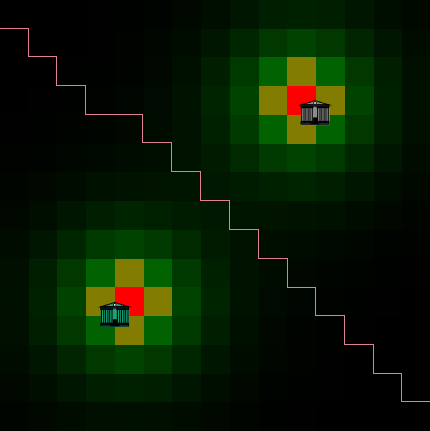
\includegraphics[width=0.49\linewidth]{Figures/Lutecia/ex_setup.png}
	%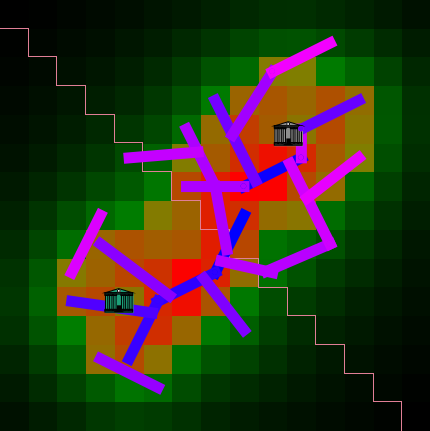
\includegraphics[width=0.49\linewidth]{Figures/Lutecia/ex_reg_infra50.png}
	%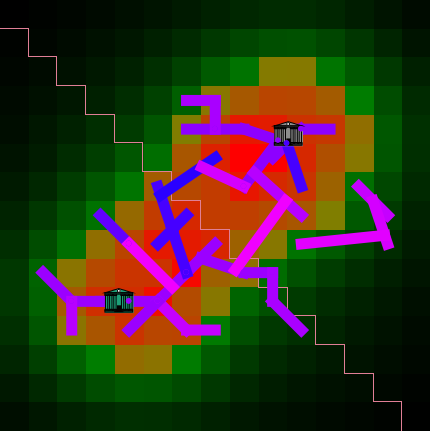
\includegraphics[width=0.49\linewidth]{Figures/Lutecia/ex_maxcollabcost_infra50.png}
	%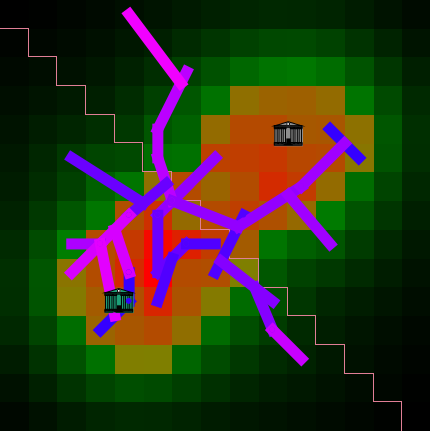
\includegraphics[width=0.49\linewidth]{Figures/Lutecia/ex_mincollabcost_infra50.png}
	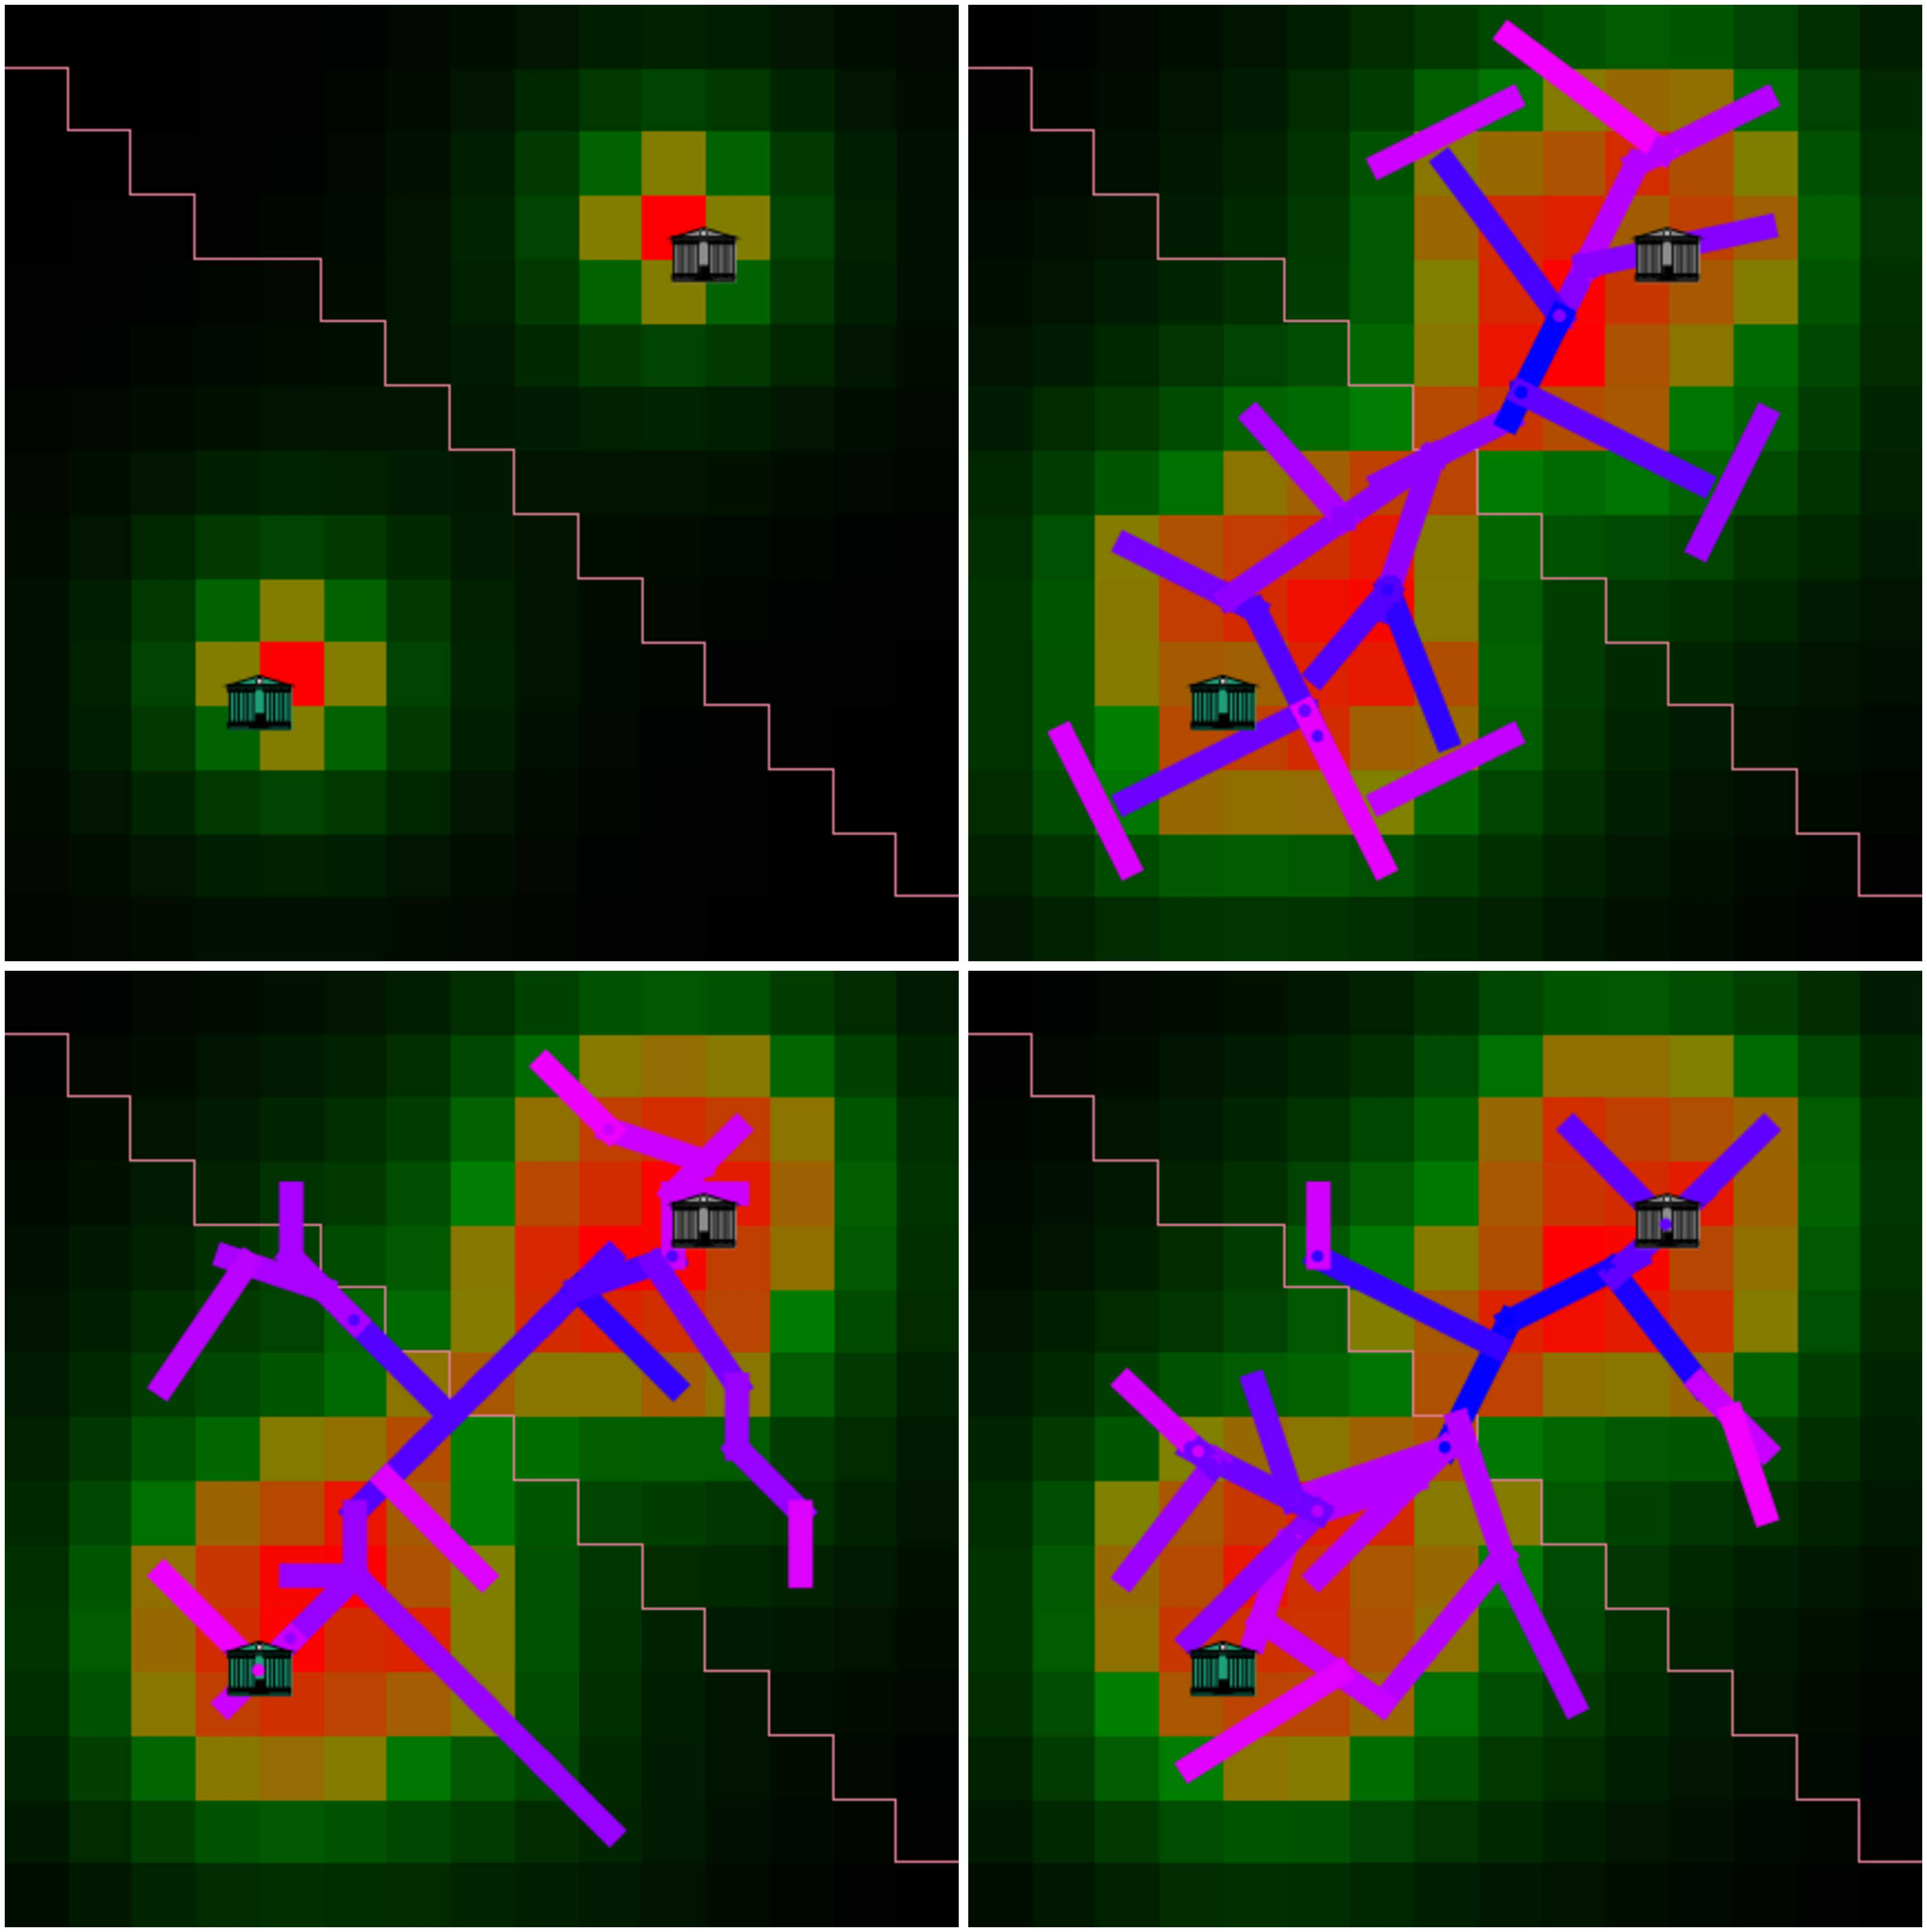
\includegraphics[width=\linewidth]{Figures/Final/7-3-3-fig-lutecia-governance.jpg}
	\caption[Network topologies obtained for different levels of governance][Formes de réseau obtenues pour différents niveaux de gouvernance]{\textbf{Network topologies obtained for different levels of governance.} The model is initialized on a symmetric synthetic configuration with two centers (\textit{Top Left}). Parameters for the evolution of land-use are $\gamma_A = \gamma_E = 0.8 ; \beta = 2 ; \lambda = 0.001 ; \alpha = 0.16$, and for network evolution $l_r = 2$ and a discrete choices game. The evolution is stopped at fixed stock $S = 50$ and the heuristic exploration done for $N_I = 200$. (\textit{Top Right}) Regional decision level ($\xi = 1$); (\textit{Bottom Left}) Local decision level ($\xi = 0$) and low level of collaboration, obtained with a high cost of cooperation $J=0.005$; (\textit{Bottom Right}) Local level and high level of collaboration, with $J=0$.\label{fig:lutecia:governance}}{\textbf{Formes de réseau obtenues pour différents niveaux de gouvernance.} Le modèle est initialisé sur une configuration synthétique symétrique à deux centres (\textit{Haut gauche}). Les paramètres pour l'évolution de l'usage du sol sont $\gamma_A = \gamma_E = 0.8 ; \beta = 2 ; \lambda = 0.001 ; \alpha = 0.16$, et pour l'évolution du réseau $l_r = 2$ et un jeu à choix discrets. L'évolution est stoppée à stock constant $S = 50$ et l'exploration heuristique faite pour $N_I = 200$. (\textit{Haut droite}) Niveau de décision régional ($\xi = 1$) ; (\textit{Bas gauche}) Niveau local ($\xi = 0$) et bas niveau de collaboration, obtenu avec un fort coût de coopération $J=0.005$ ; (\textit{Bas droite}) Niveau local et haut niveau de collaboration, avec $J=0$.\label{fig:lutecia:governance}}
\end{figure}
%%%%%%%%%%%%



\paragraph{Co-evolution}{Co-évolution}


\bpar{
In a last stylized experiment, we propose to study more directly the effect of co-evolution, in particular on land-use variables. Therefore, we consider again the previous bi-centric configuration, with a disequilibrium of population and employments between the two centers (in practice with a rate of 2), and different proximities (close, at a distance of $0.4 \cdot K$, and far, at a distance of $K$). We fix a random local governance (choice of only one constructor with a probability proportional to employments) and the land-use and network parameters\footnote{We take here $\gamma_A = 0.9, \gamma_E = 0.65, \lambda = 0.005, \beta = 1.8, \alpha = 0.1, l_r = 1, v_0 = 6$.}, and we study the influence of the decision level $\xi$ on (i) the total accessibility gain between the initial and the final state, expressed as a rate $\frac{X(t_f)}{X(t_0)}$; and (ii) the evolution of relative accessibility between the two centers, given by $\frac{X_0(t_f)}{X_0(t_0)} / \frac{X_1(t_f)}{X_1(t_0)}$. The first indicators allows to understand the global benefit, whereas the second expresses the inequality between the centers (for example, is the weakest center drained by the more important, or does it benefit from it).
}{
Dans une dernière expérience stylisée, nous proposons d'étudier plus directement l'effet de la co-évolution, notamment sur les variables d'usage du sol. Pour cela, nous reprenons la configuration bicentrique précédente, avec un déséquilibre de population et d'emplois entre les deux centres (en pratique avec un rapport de 2), et une proximité variable (proches, à une distance de $0.4\cdot K$, et lointains, à une distance de $K$). Nous fixons une gouvernance locale aléatoire (choix d'un seul constructeur avec une probabilité proportionnelle aux emplois) et les paramètres d'usage du sol et de réseau\footnote{Nous prenons ici $\gamma_A = 0.9, \gamma_E = 0.65, \lambda = 0.005, \beta = 1.8, \alpha = 0.1, l_r = 1, v_0 = 6$.}, et nous étudions l'influence du niveau de décision $\xi$ sur (i) le gain d'accessibilité total entre l'instant initial et l'instant final, exprimé comme un rapport $\frac{X(t_f)}{X(t_0)}$ ; et (ii) l'évolution de l'accessibilité relative entre les deux centres, donnée par $\frac{X_0(t_f)}{X_0(t_0)} / \frac{X_1(t_f)}{X_1(t_0)}$. Le premier indicateur permet de comprendre le bénéfice global, tandis que le second exprime l'inégalité entre les centres (par exemple, le centre le plus faible est-il drainé par le plus important, ou bénéficie-t-il de celui-ci).
}


\bpar{
Results of the experiment are given in Fig.~\ref{fig:lutecia:coevol}. The behavior of the accessibility gain unveil a direct effect of co-evolution processes: in the case of distant centers, the effect of $\xi$ on it is inverted when we add the evolution of land-use. In the case of a network evolving alone, a local decision is optimal for total accessibility, whereas in the case of a co-evolution of processes, the optimal is at a fully regional decision. We interpret this stylized fact as the existence of a need for coordination for the success of a coupled evolution of the transportation network and land-use, what can be put in correspondence with the concept of TOD seen in chapter~\ref{ch:thematic}. In the case of close centers, the regional decision is always optimal, corresponding then to a more integrated metropolitan area. The variation of the relative accessibility are to low to conclude on the evolution of inequalities between the centers in the case of a coupled evolution.
}{
Les résultats de l'expérience sont donnés en Fig.~\ref{fig:lutecia:coevol}. Le comportement du gain d'accessibilité révèle un effet direct des processus de co-évolution : dans le cas de centres distants, l'effet de $\xi$ sur celui-ci s'inverse lorsqu'on ajoute l'évolution de l'usage du sol. Dans le cas d'un réseau qui évolue seul, une décision locale est optimale pour l'accessibilité totale, tandis que dans le cas d'une co-évolution des processus, l'optimal est à une décision purement régionale. Nous interprétons ce fait stylisé comme l'existence d'un besoin de coordination pour la réussite d'une évolution couplée du réseau de transport et de l'usage du sol, ce qui peut être mis en relation avec le concept du TOD vu au chapitre~\ref{ch:thematic}. Dans le cas de centres proches, la décision régionale est toujours optimale, correspondant alors à une métropole plus intégrée. Les variations de l'accessibilité relative sont trop faibles pour conclure sur l'évolution des inégalités entre les centres dans le cas d'une évolution couplée.
}


\bpar{
Thus, this last experiment reveals indeed the existence of ``co-evolution effects'', in the emergence of a need for regional coordination in the case of a coupled evolution.
}{
Ainsi, cette dernière expérience révèle bien l'existence ``d'effets de co-évolution'', dans l'émergence d'un besoin de coordination régionale dans le cas d'une évolution couplée.
}


%%%%%%%%%%%%
\begin{figure}
	%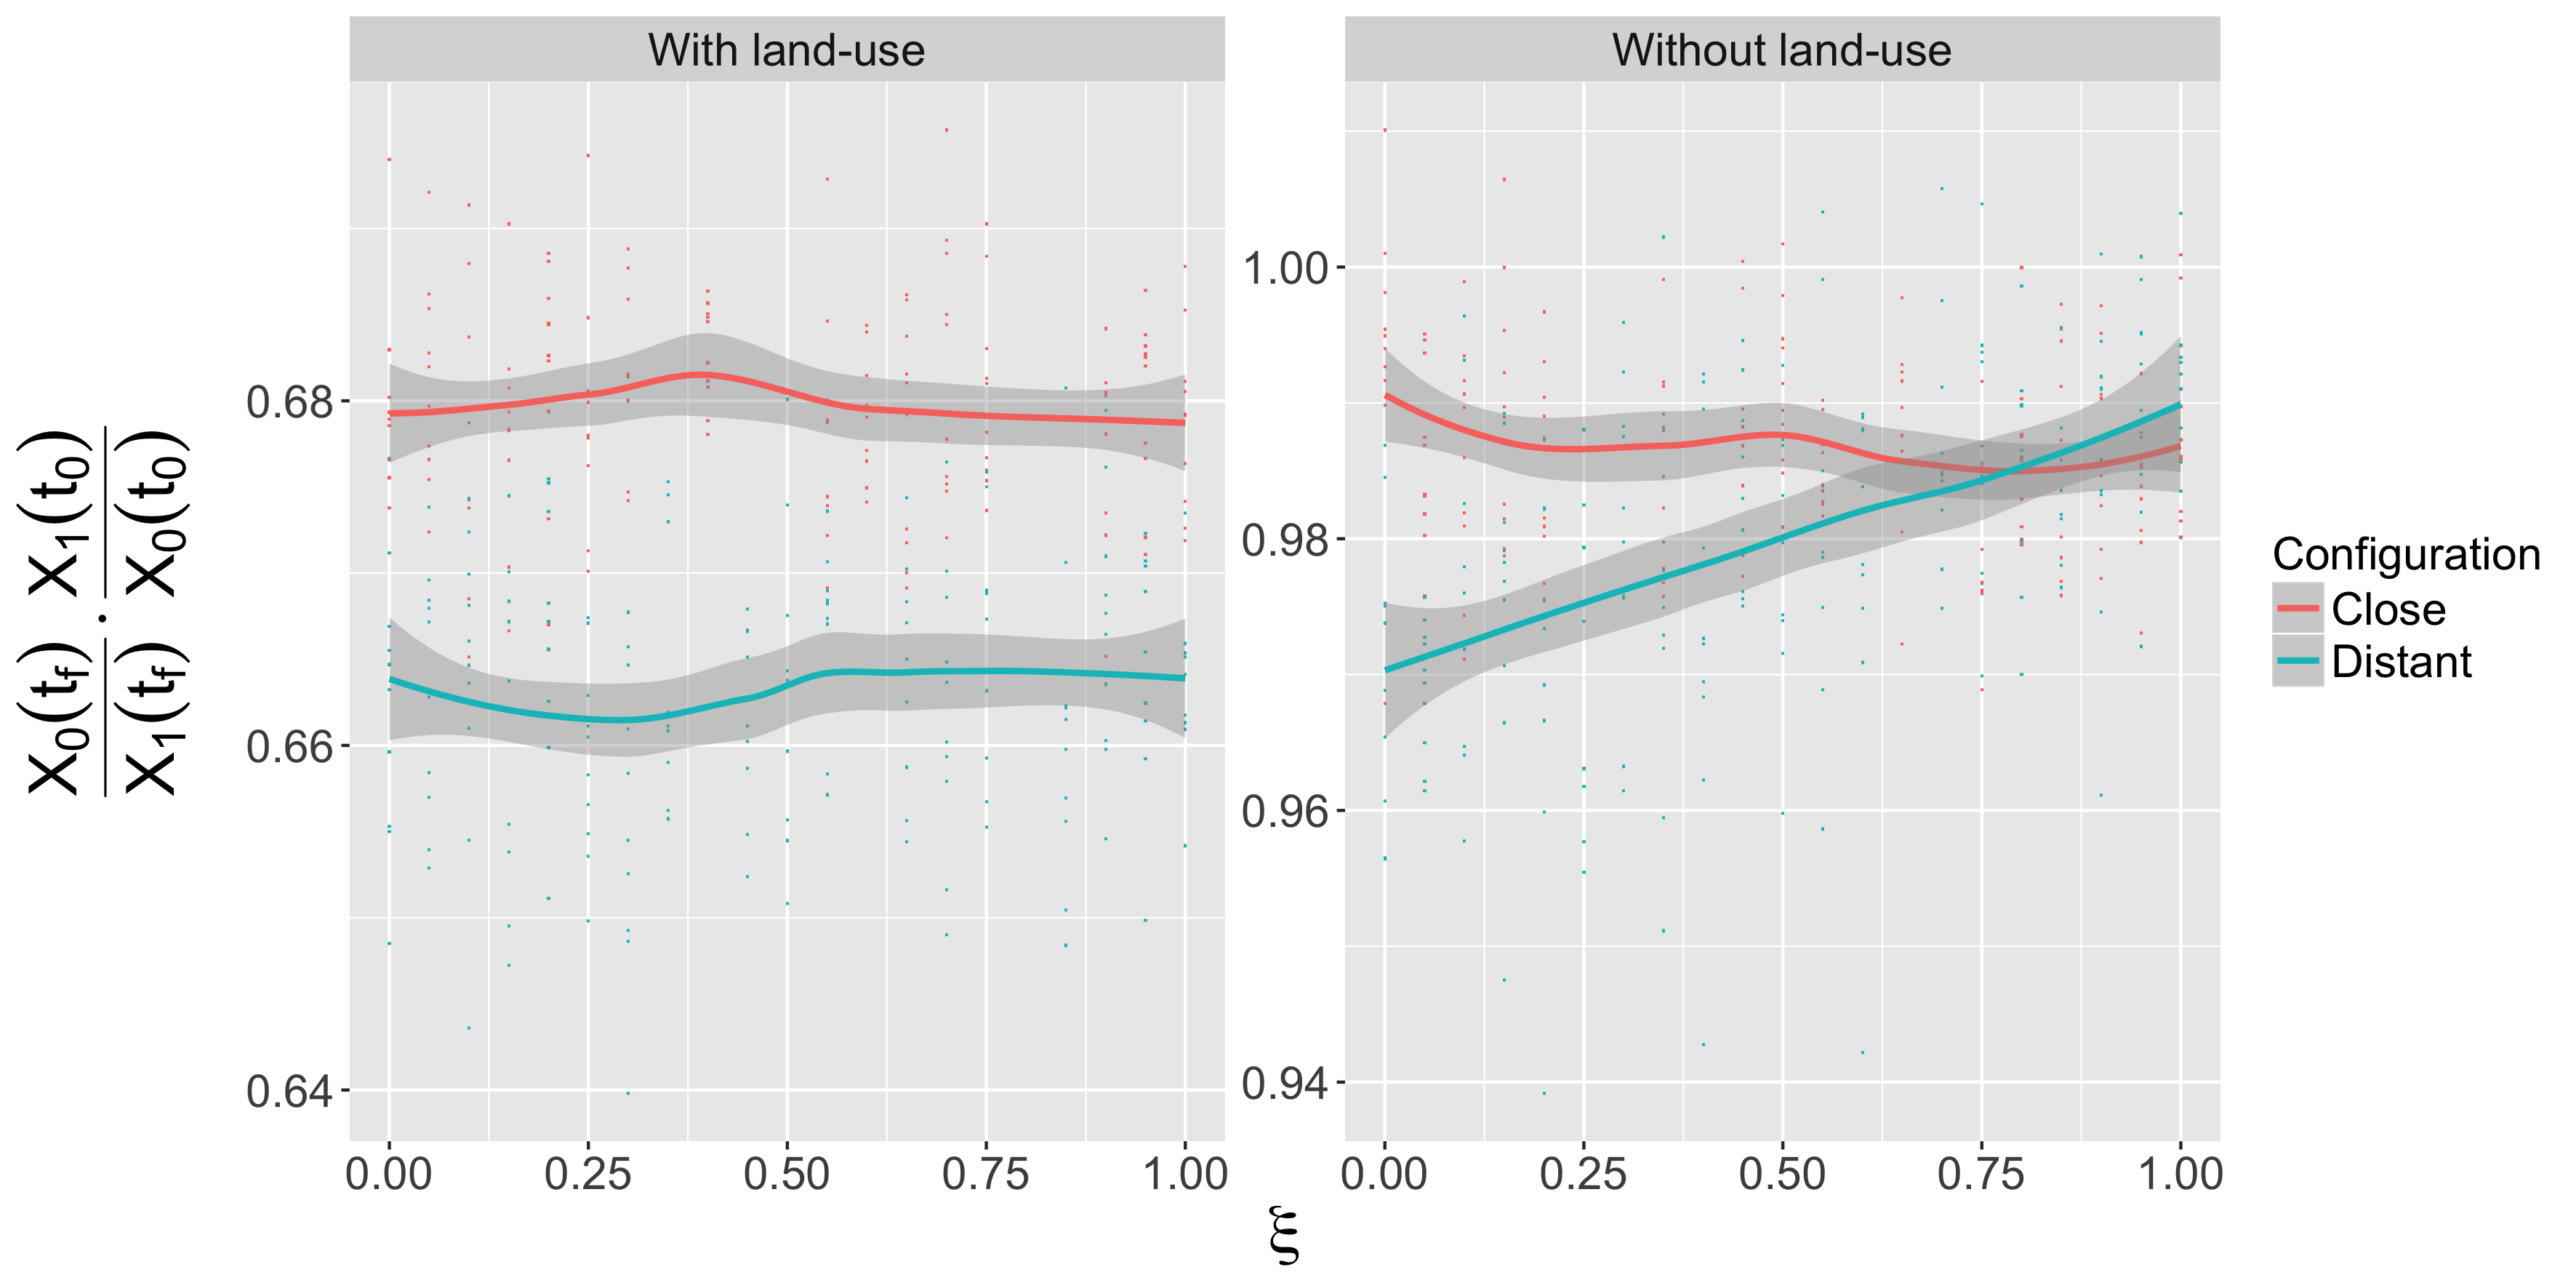
\includegraphics[width=\linewidth]{Figures/Lutecia/accessbalance.png}\\
    %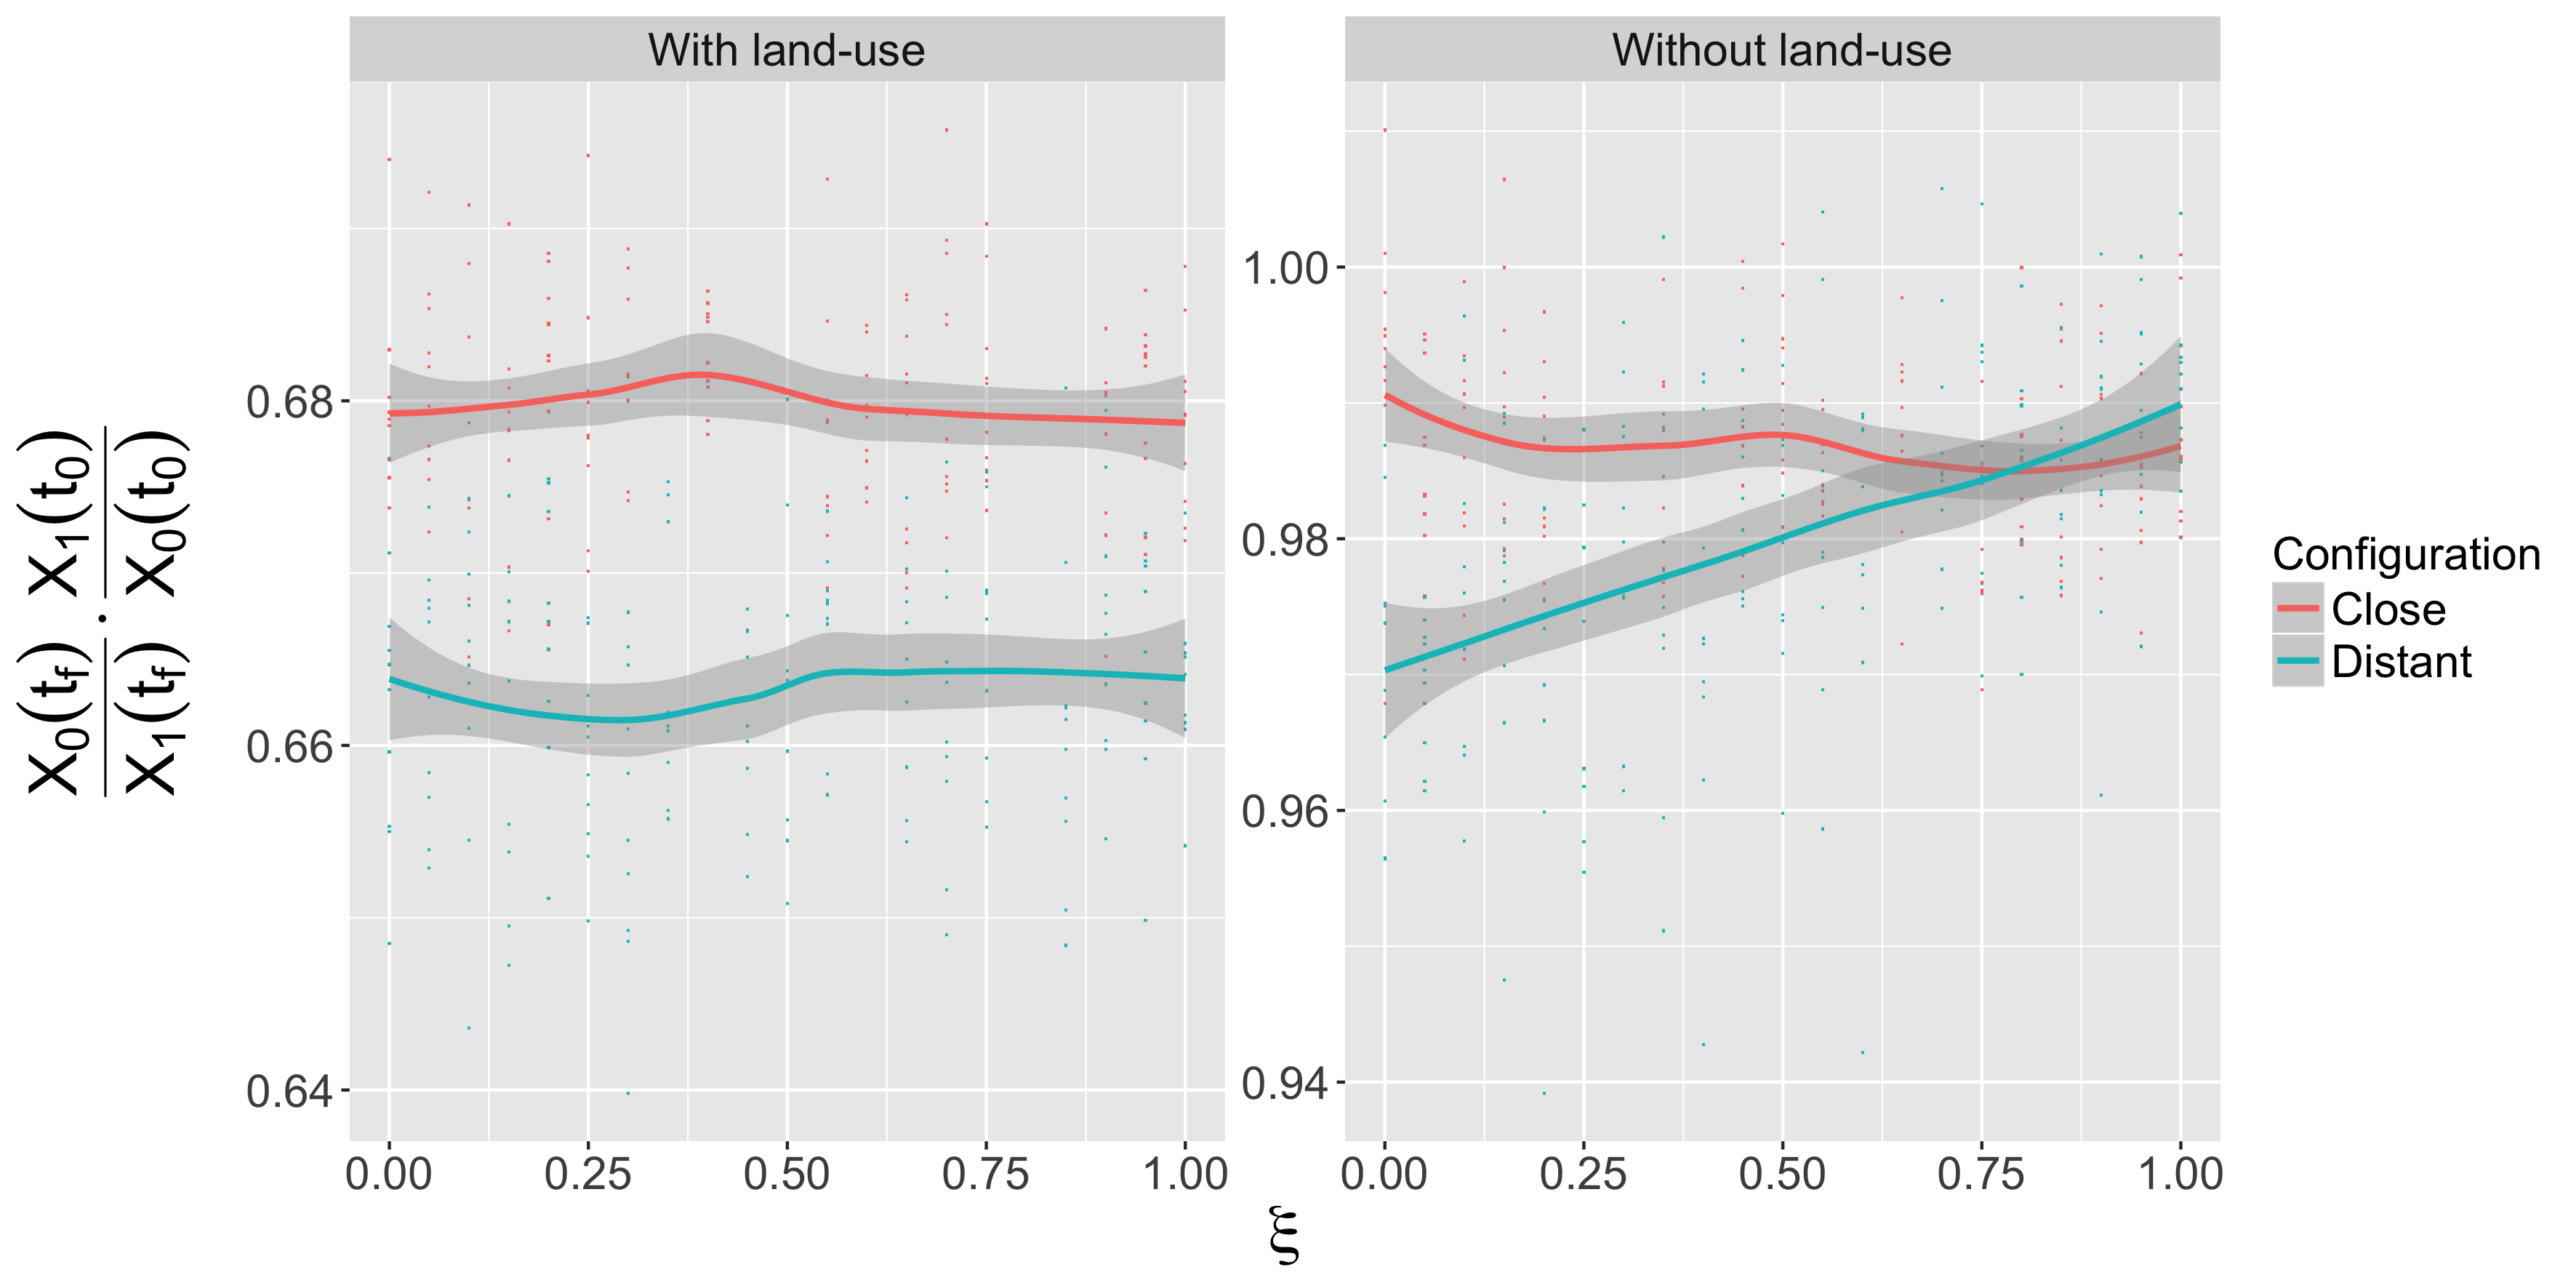
\includegraphics[width=\linewidth]{Figures/Lutecia/accesstot.png}
	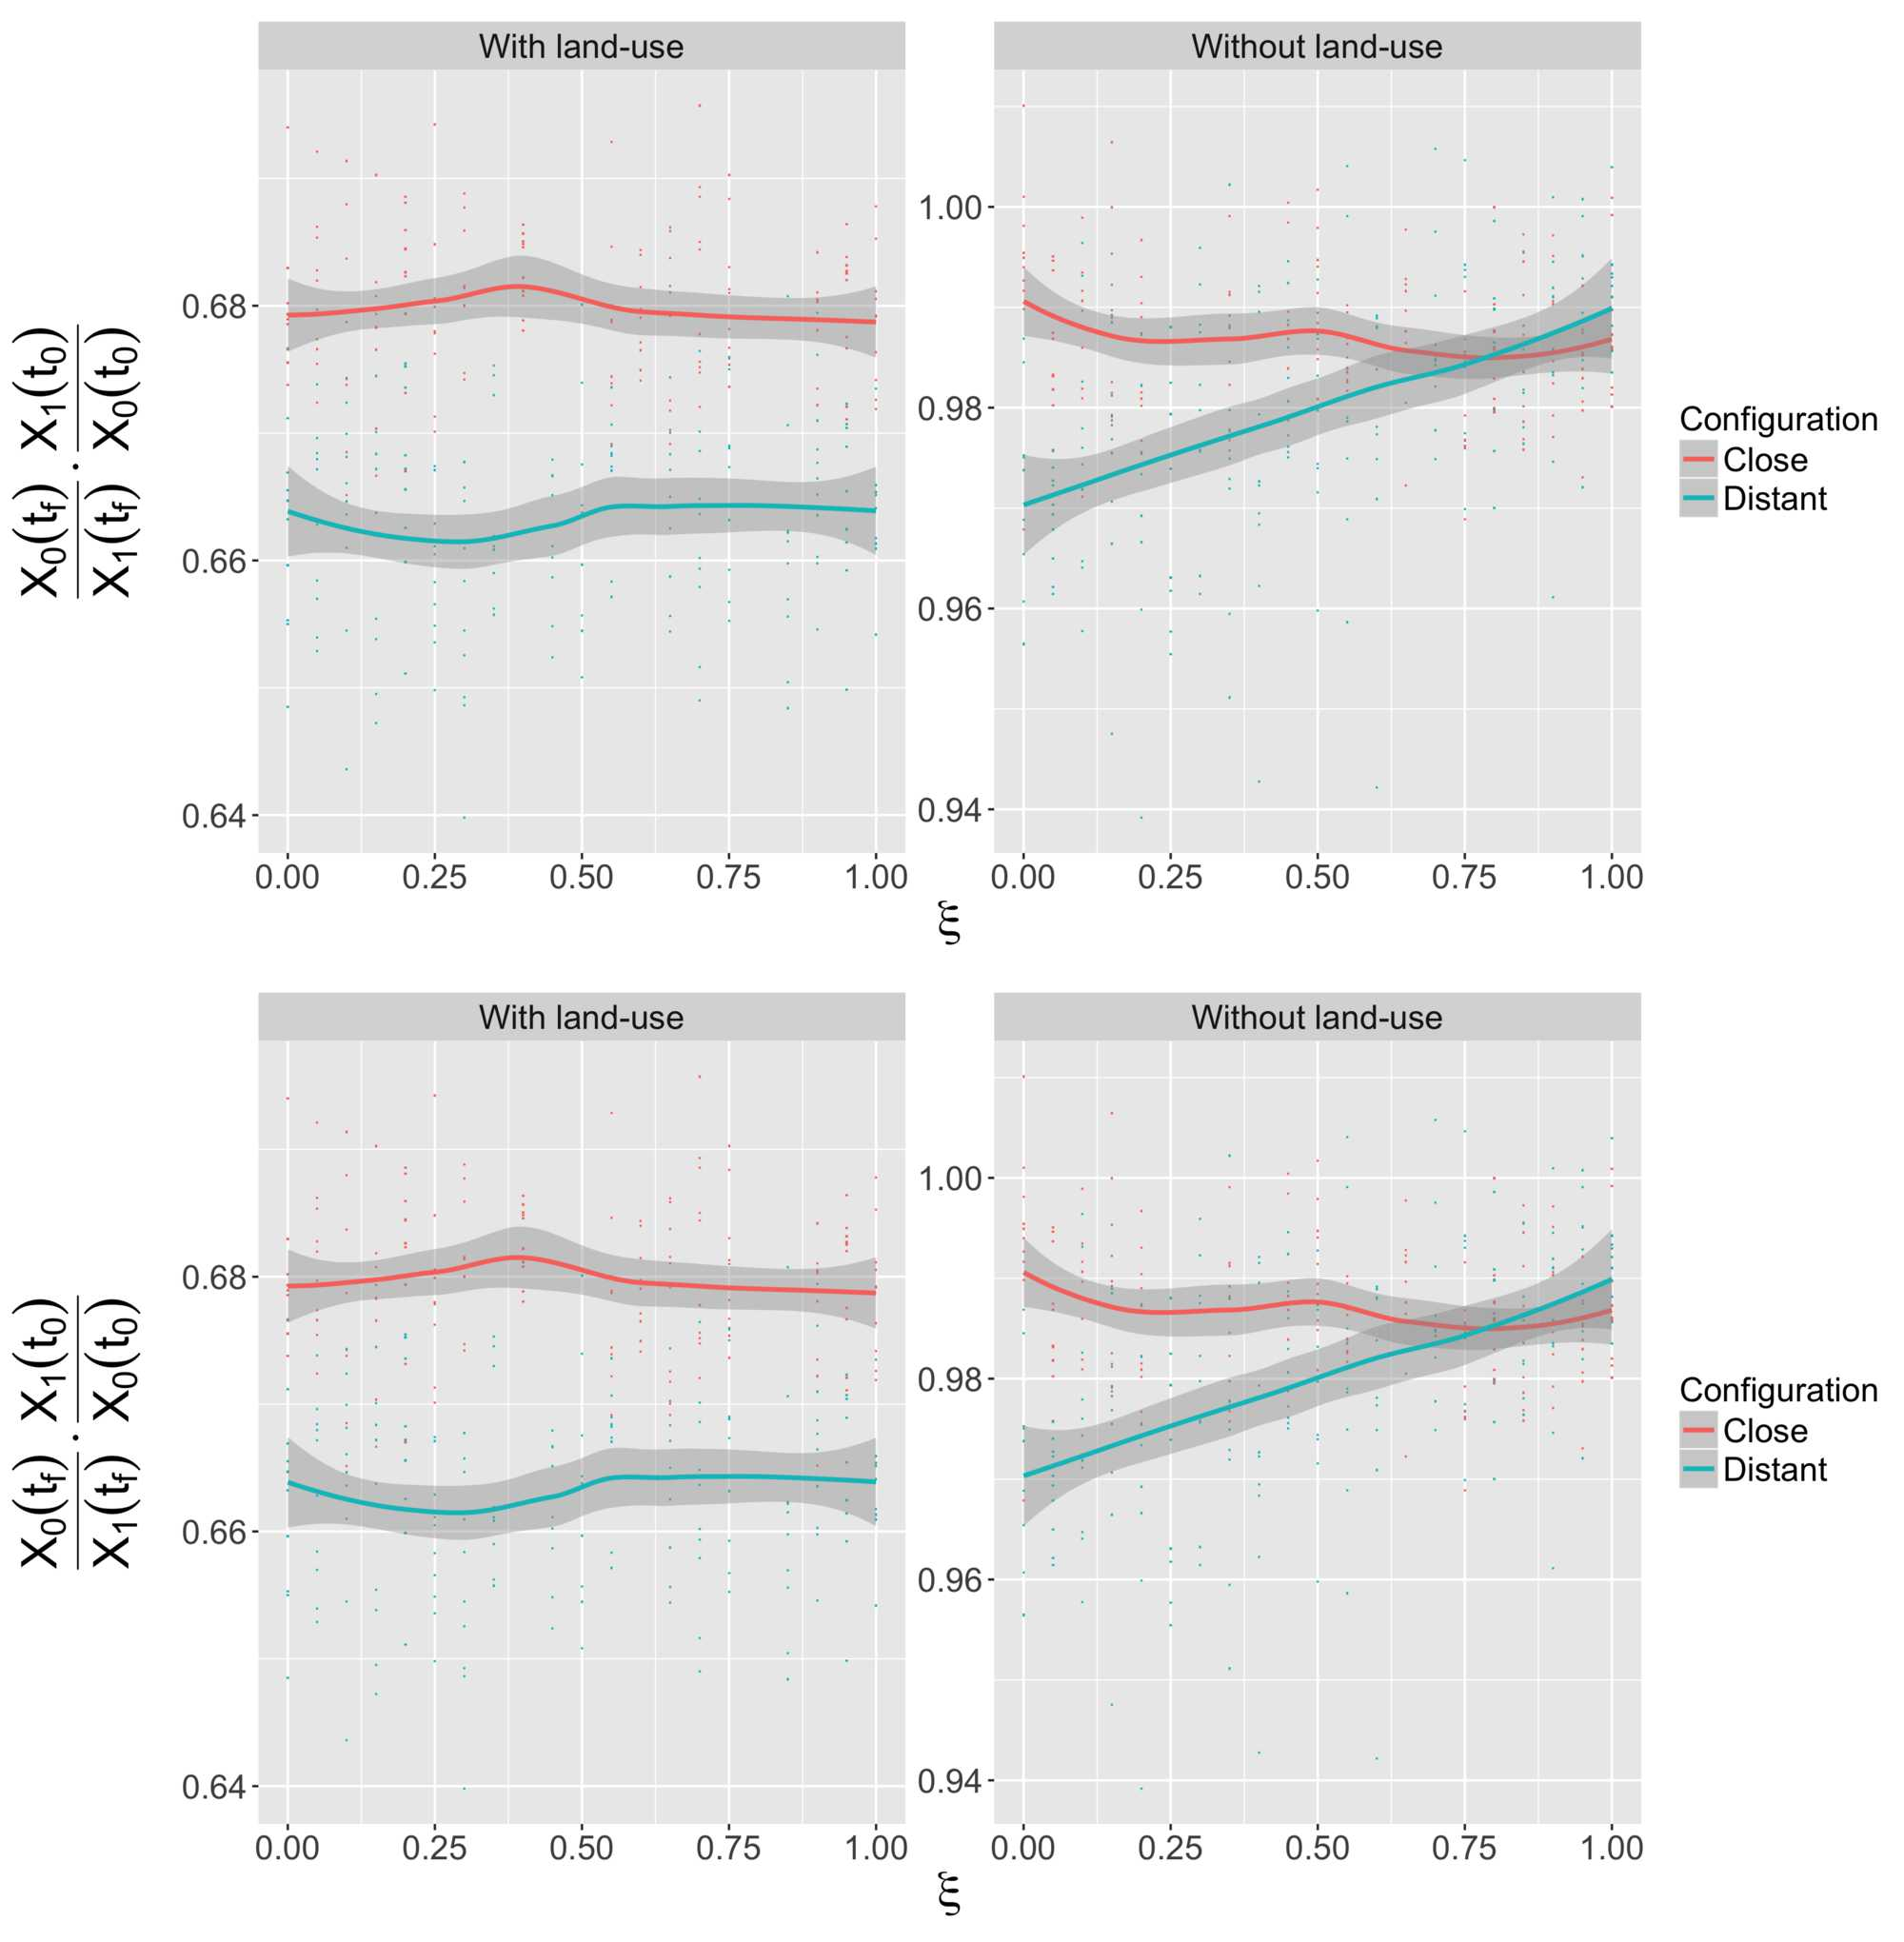
\includegraphics[width=\linewidth]{Figures/Final/7-3-3-fig-lutecia-coevol.jpg}
	\caption[Impact of co-evolution on accessibility in the Lutecia model][Impact de la co-évolution sur l'accessibilité dans le modèle Lutecia]{\textbf{Impact of co-evolution on accessibility in the Lutecia model.} We proceed to 10 repetitions with fixed parameters $\gamma_A = 0.9, \gamma_E = 0.65, \lambda = 0.005, \beta = 1.8, \alpha = 0.1, l_r = 1, v_0 = 6$, for a random local governance, and an evolution with constant stock $S=20$. We compare the evolution with network only (without land-use) and with co-evolution, for the close and distant configurations. (\textit{Top}) Evolution of the relative accessibility between centers, with and without land-use (columns) for the two configurations (colours); (\textit{Bottom}) Total accessibilty gain.\label{fig:lutecia:coevol}}{\textbf{Impact de la co-évolution sur l'accessibilité dans le modèle Lutecia.} Nous effectuons 10 répétitions avec les paramètres fixés $\gamma_A = 0.9, \gamma_E = 0.65, \lambda = 0.005, \beta = 1.8, \alpha = 0.1, l_r = 1, v_0 = 6$, pour une gouvernance locale aléatoire, et une évolution à stock constant $S=20$. Nous comparons l'évolution avec réseau uniquement (sans usage du sol) et avec co-évolution, pour les configurations proches et distantes. (\textit{Haut}) Évolution de l'accessibilité relative entre les centres, avec et sans usage du sol (colonnes) pour les deux configurations (couleurs) ; (\textit{Bas}) Gain d'accessibilité totale.\label{fig:lutecia:coevol}}
\end{figure}
%%%%%%%%%%%%





%%%%%%%%%%%%%%%%%%%%
\subsection{Application to Pearl River Delta}{Application au Delta de la Rivière des Perles}


\bpar{
It was suggested by \cite{liao2017ouverture} that a sort of multi-level governance recently emerged in China, in the context of economic activities. We try with our model to test the relevance of this paradigm regarding the urban structure of the MCR.
}{
Il a été suggéré par \cite{liao2017ouverture} qu'une forme de gouvernance multi-niveau a récemment émergé en Chine, dans le contexte des activités économiques. Nous tentons par notre modèle de tester la pertinence de ce paradigme au regard de la structure urbaine de la MCR.
}






%
%
\subsubsection{Model setup}{Initialisation du modèle}

\bpar{
We work on a simplified raster configuration (5km cells) for population in Pearl River Delta, and on the stylized freeway network. We choose to consider only the road network since, following \cite{hou2011transport}, it has been the main driver of changes in accessibility patterns compared to railway network which accelerated development is recent. Networks are stylized from the plan given by~\cite{hou2011transport} which reproduces official documents of Guangdong province in 2010. We thus consider the freeway network in 2010 and the one planned at this time. Employment data are given for 2010 by~\cite{swerts2017database} at the level of cities. They are here uniformly distributed for each city in the simplified raster. The Fig.~\ref{fig:lutecia:ex-prd} illustrates the stylized configuration for Pearl River Delta.
}{
Nous travaillons sur une configuration raster simplifiée (cellules de 5km) pour la population du Delta de la Rivière des Perles, ainsi que sur le réseau d'autoroute stylisé. Nous considérons le réseau routier uniquement puisque, selon \cite{hou2011transport}, il s'agit du moteur principal des changements dans les motifs d'accessibilité en comparaison au réseau ferré dont le développement accéléré est récent. Les réseaux sont stylisés à partir du plan donné par~\cite{hou2011transport} qui reproduit les documents officiels de la province du Guangdong en 2010. Nous considérons ainsi le réseau autoroutier en 2010 et celui planifié à cette époque. Les données des emplois sont fournies en 2010 par~\cite{swerts2017database} au niveau des communes. Ils sont distribués ici uniformément pour chaque ville dans le raster simplifié. La Fig.~\ref{fig:lutecia:ex-prd} illustre la configuration stylisée pour le Delta de la Rivière des Perles.
}


%
%We show in Fig.~\ref{fig:ex-prd} an illustration of the stylized setup of the model and of its outcome with standard parameter values.


%%%%%%%%%%%%%%%%%%%%
\begin{figure}
%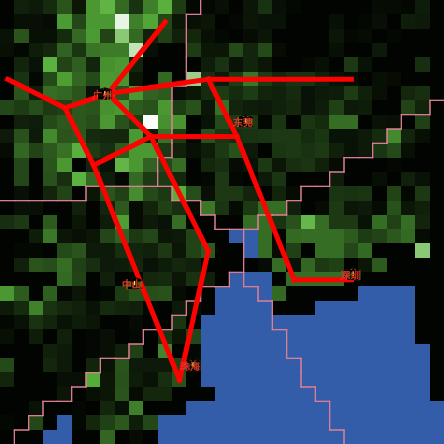
\includegraphics[width=0.49\linewidth]{Figures/Lutecia/exrun_2_tick0}
%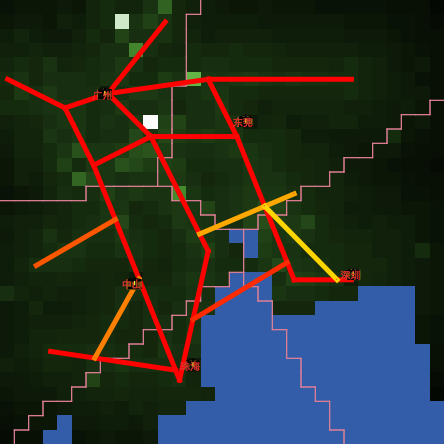
\includegraphics[width=0.49\linewidth]{Figures/Lutecia/exrun_2_tick6}
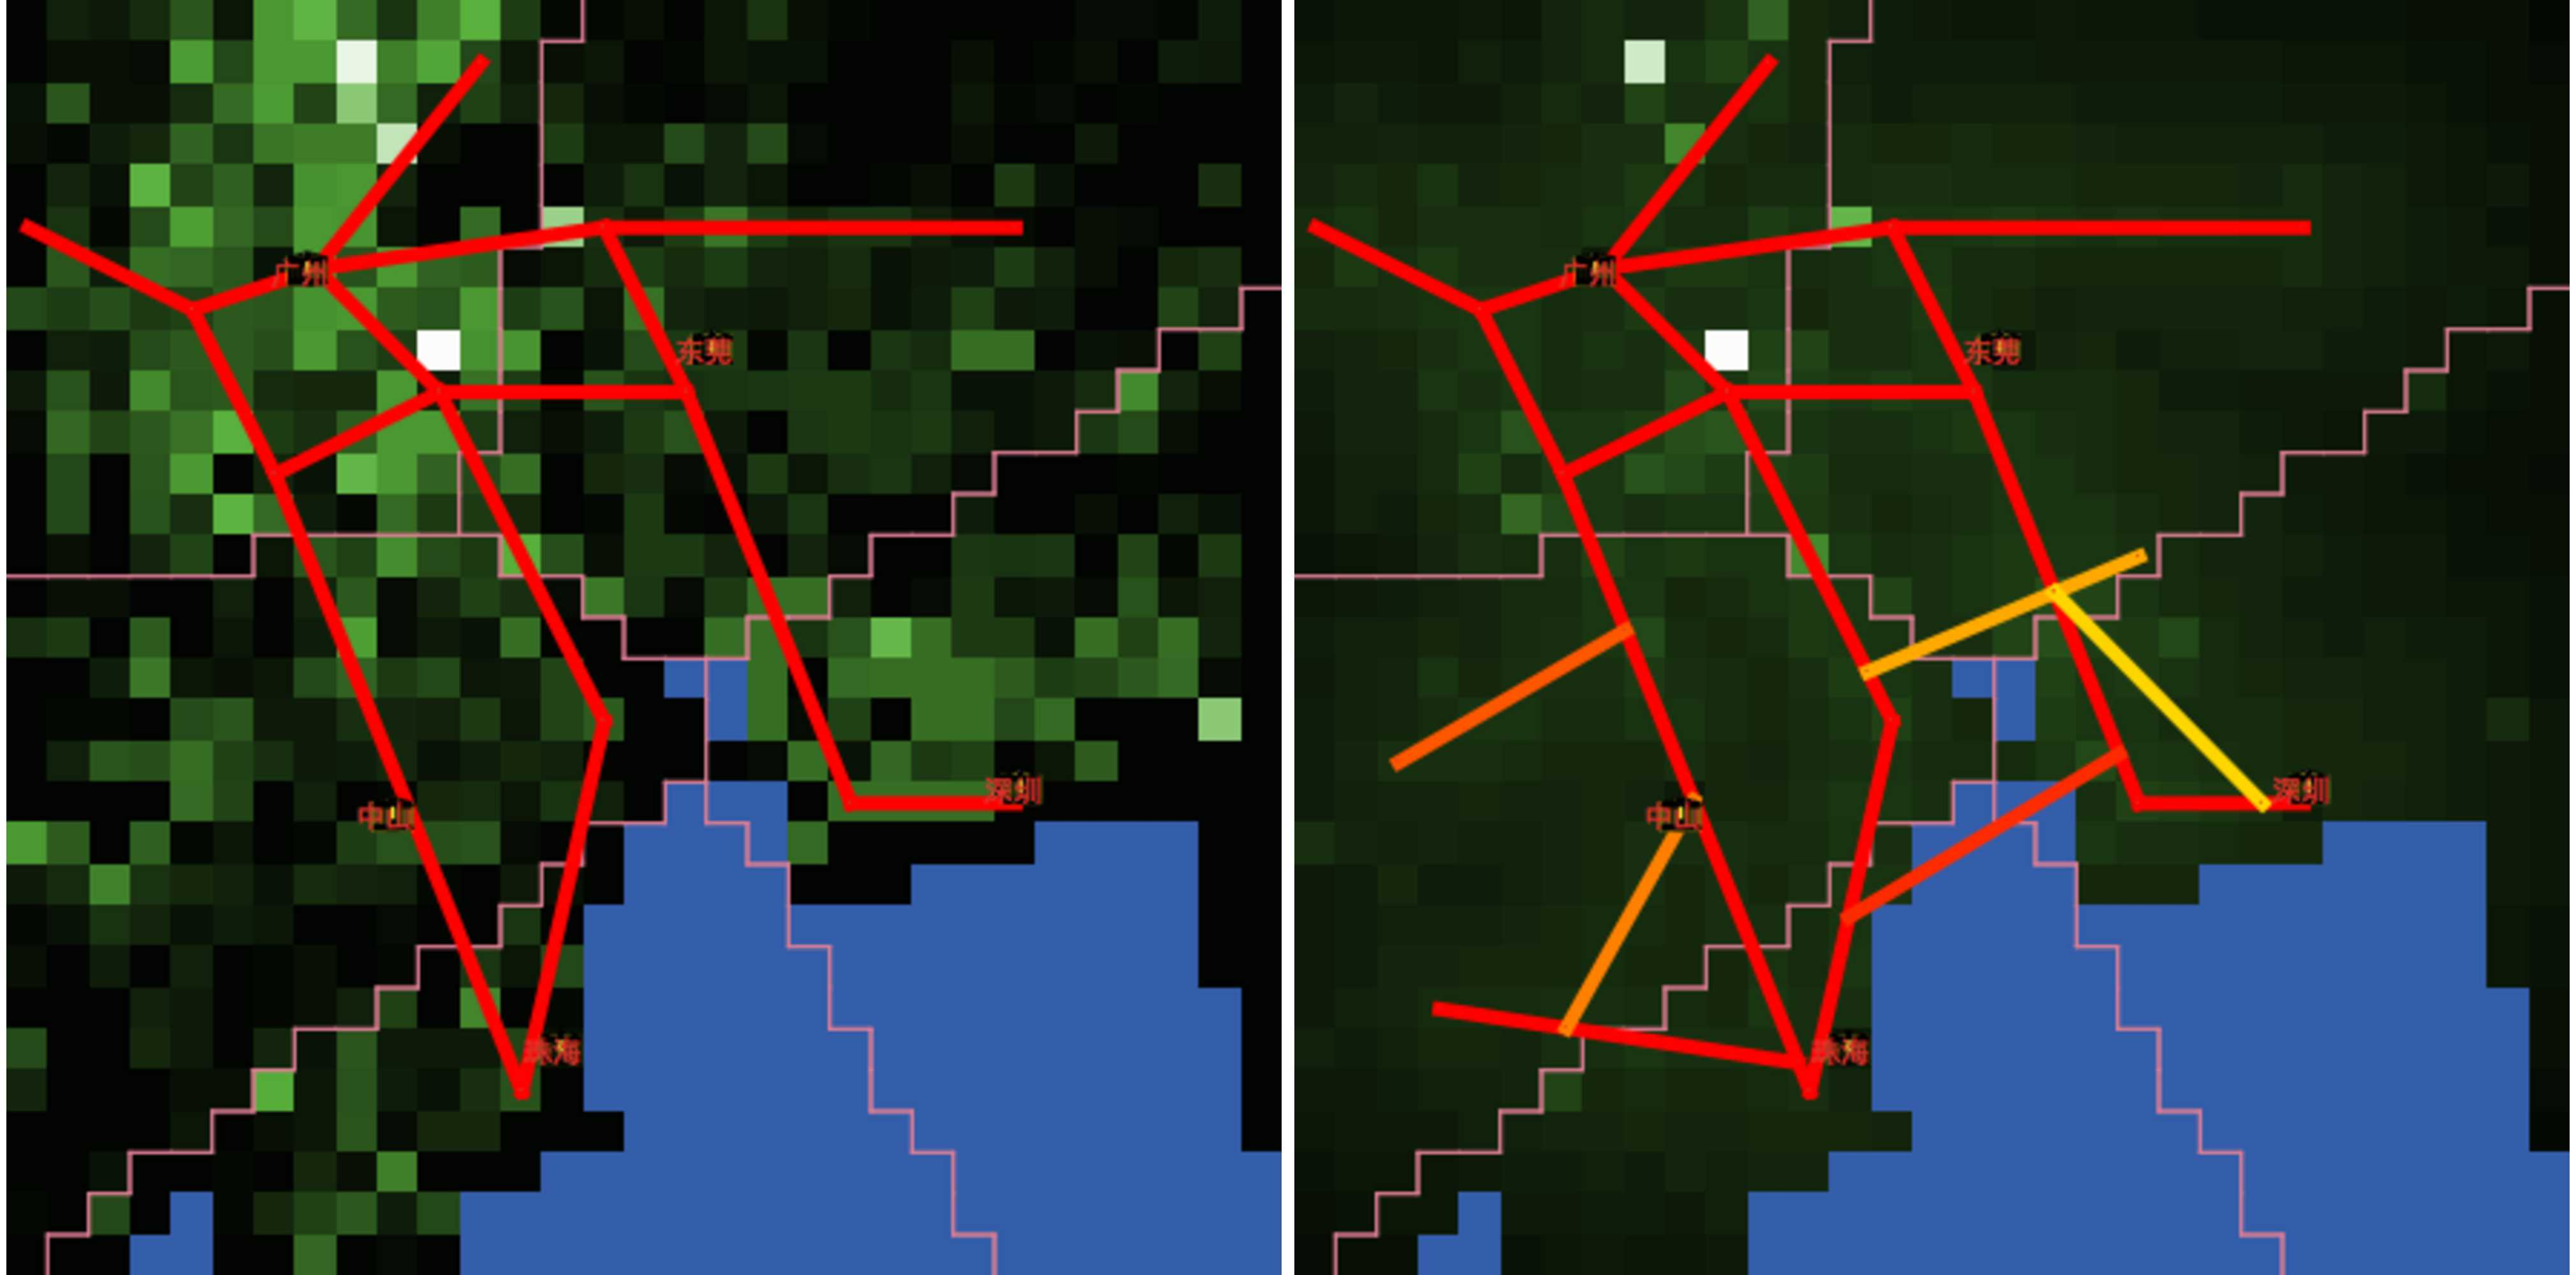
\includegraphics[width=\linewidth]{Figures/Final/7-3-3-fig-lutecia-ex-prd.jpg}
\caption[Application of Lutecia to Pearl River Delta][Application de Lutecia au Delta de la Rivière des Perles]{\textbf{Example of application to Pearl River Delta.} (\textit{Left}) Initialization with the 2010 population raster, aggregated at the 5km resolution, and the simplified freeway network; (\textit{Right}) State after 6 time steps ($\alpha = 1$).\label{fig:lutecia:ex-prd}}{\textbf{Exemple d'application au Delta de la Rivière des Perles.} (\textit{Gauche}) Initialisation avec le raster de population 2010, agrégé à la résolution 5km, et le réseau autoroutier simplifié ; (\textit{Droite}) Etat après 6 pas de temps ($\alpha = 1$).\label{fig:lutecia:ex-prd}}
\end{figure}
%%%%%%%%%%%%%%%%%%%%





\subsubsection{Calibration procedure}{Procédure de calibration}


\bpar{
To apply such a complex model to a semi-real situation, one must be particularly careful. It is important to choose the adequate processes and level of granularity to reproduce. In particular, our model is not aimed at producing particularly accurate land-use patterns, but uses their approximation as the basis of network growth, which qualitative evolution and the corresponding qualitative patterns in governance processes. We propose therefore to ``calibrate'' on the shape of a given infrastructure, in the sense of determining parameter configurations for which in probability the successive built pieces of infrastructure are the closest to pieces of the target infrastructure. 
}{
Lors de l'application d'un modèle si complexe à une situation semi-réelle, il faut rester vigilant. Il est important de choisir les processus adéquats ainsi que le niveau de granularité à reproduire. En particulier, notre modèle produit des motifs d'usage du sol relativement précis, mais utilise leur approximation comme base de la croissance du réseau, dont l'évolution qualitative permet d'informer sur les processus de gouvernance. Nous proposons pour cela de ``calibrer'' sur la forme d'une infrastructure donnée, au sens de déterminer des configurations de paramètres pour lesquelles en probabilité les morceaux successifs d'infrastructure sont les plus proches d'une infrastructure visée.
}


\bpar{
To calibrate on the network produced by the simulation, it must be compared to a reference network. This is however a difficult problem, as different proximity measures with different significations can be used. Geometrical measures focus on the spatial proximity of networks. For a network $(E,V)=((e_j),(v_i))$, a node-based distance is given by $\sum_{i \neq i'} d^2 \left(v_i,v_{i'}\right)$. A more accurate measure which is not biased by intermediate nodes is given by the cumulated area between each pair of edges $\sum_{j \neq j'} A \left(e_j,e_{j'}\right)$ (not a distance in the proper sense) where $A(e,e')$ is the area of the closed polygon formed by joining link extremities. We consider the latest for the calibration.
}{
Pour calibrer sur les réseaux produits par la simulation, il s'agit de comparer à un réseau de référence. C'est un problème difficile, puisque différentes mesures de proximité avec différentes significations peuvent être utilisées. Les mesures géométriques s'intéressent à la proximité spatiale des réseaux. Pour un réseau $(E,V)=((e_j),(v_i))$, une distance basée sur les noeuds est donnée par $\sum_{i \neq i'} d^2 \left(v_i,v_{i'}\right)$. Une mesure plus précise qui n'est pas biaisée par d'éventuels noeuds intermédiaires est donnée par l'aire cumulée entre chaque paire de liens $d_A = \sum_{j \neq j'} A \left(e_j,e_{j'}\right)$ (il ne s'agit pas d'une distance à proprement parler), où $A(e,e')$ est l'aire du polygone fermé constitué en reliant les sommets des liens. Nous considérerons cette dernière pour la calibration.
}




\subsubsection{Calibration}{Calibration}


\bpar{
The experiments we do are with a fixed land-use, since the required level of detail for more ancient or recent data, or even projections, for population and employments, is not allowed by the data we had access to.
}{
Les expériences que nous menons sont à usage du sol fixé, le niveau de détail requis pour des données plus anciennes et plus récentes, voir des projections, pour la population et les emplois n'étant pas permis par les données à notre disposition.
}


\bpar{
We make governance parameters vary, including the type of game, with a fixed $l_r = 2$, and explore a Latin Hypercube Sampling of 4000 points in this parameter space, with 10 repetitions of the model for each point. The two experiments we performed correspond to different target configurations:
\begin{itemize}
	\item no initial network and the 2010 network as a target, in the spirit of extrapolating the most probable governance configuration which led to the current configuration;
	\item initial network as the 2010 network, and planned network as target: extrapolation of the governance configuration for the planning.
\end{itemize}
}{
Nous faisons varier les paramètres de gouvernance, incluant le type de jeu, avec $l_r = 2$ fixé, et explorons un échantillonnage LHS de 4000 points dans l'espace de ces paramètres, avec 10 répétitions du modèle pour chaque point. Les deux expériences menées correspondent à des configurations cibles différentes :
\begin{itemize}
	\item aucun réseau initial et réseau de 2010 comme cible, dans l'esprit d'extrapoler la configuration de gouvernance la plus probable ayant mené à la configuration actuelle ;
	\item réseau 2010 initial, et réseau planifié comme cible : extrapolation de la configuration de gouvernance de la planification.
\end{itemize}
}


\bpar{
We obtain qualitatively similar results for the two experiments, suggesting that there was no transition in the type of governance between the past network and the future network. Results are illustrated in Fig.~\ref{fig:lutecia:calib}. We obtain, by studying the graph of $d_A$ as a function of $\xi$, that the regional level is the most realistic to reproduce network shape. However, discrete choices and competition games have a different behavior, and the competitive game is the closest to reality when $\xi$ decreases: the relations between local actors would a priori be of a more competitive than an egoistic nature. When we study the variation of distance as a function of the observed collaboration level, we obtain an interesting inverted U-shape, i.e. that the most likely configurations are the ones where there is only collaboration, or the ones where there is no collaboration at all, but no intermediate situations. Finally, the comparison of statistical distributions of distances between target configurations and the types of games shows that the difference between the games is significant only for the real network but not for the planned network (what remains a conclusion difficult to interpret).
}{
Nous obtenons des résultats qualitativement similaires pour les deux expériences, suggérant qu'il n'y a pas eu de transition de type de gouvernance entre réseau passé et réseau futur. Les résultats sont illustrés en Fig.~\ref{fig:lutecia:calib}. On obtient, à l'étude du graphe de $d_A$ en fonction de $\xi$, que le niveau régional est le plus fidèle pour reproduire la forme du réseau. Par contre, les jeux de choix discrets et de compétition se comportent différemment, et le jeu compétitif est le plus proche de la réalité quand $\xi$ diminue : les relations entre acteurs locaux seraient a priori de nature plus compétitive qu'égoïste. Quand on étudie la variation de la distance en fonction du niveau de collaboration observé, on obtient une forme intéressante en cloche inversée, c'est-à-dire que les situations les plus probables sont soit celles où il n'y a que de la collaboration, soit celles où il n'y en a pas du tout, mais pas de situations intermédiaires. Enfin, la comparaison des distributions statistiques des distances entre les configurations cibles et les types de jeux montre que la différence entre les jeux n'est considérable que pour le réseau réel mais pas le réseau planifié (ce qui reste une conclusion difficile à interpréter).
}



%%%%%%%%%%%%%%%
\begin{figure}
	%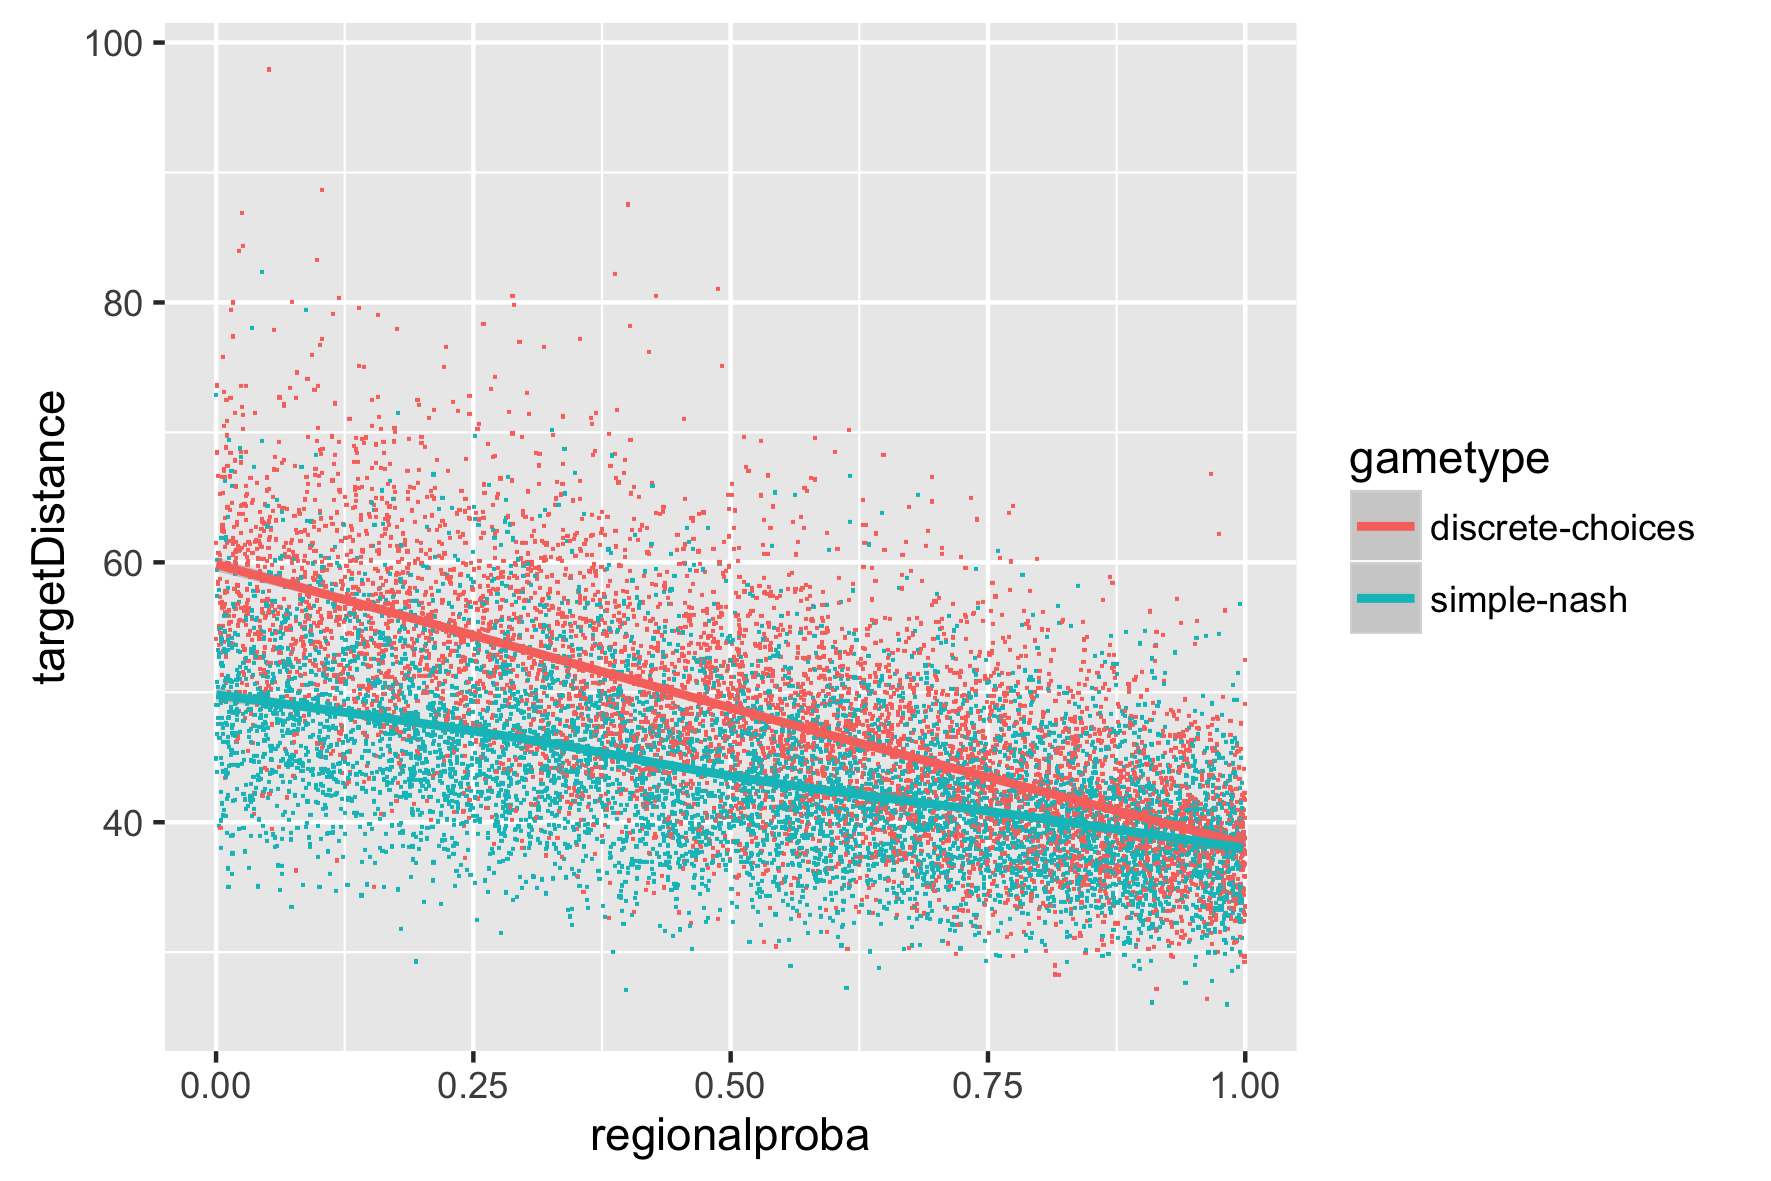
\includegraphics[width=0.49\linewidth]{Figures/Lutecia/regional-distance_colorgametype.png}
	%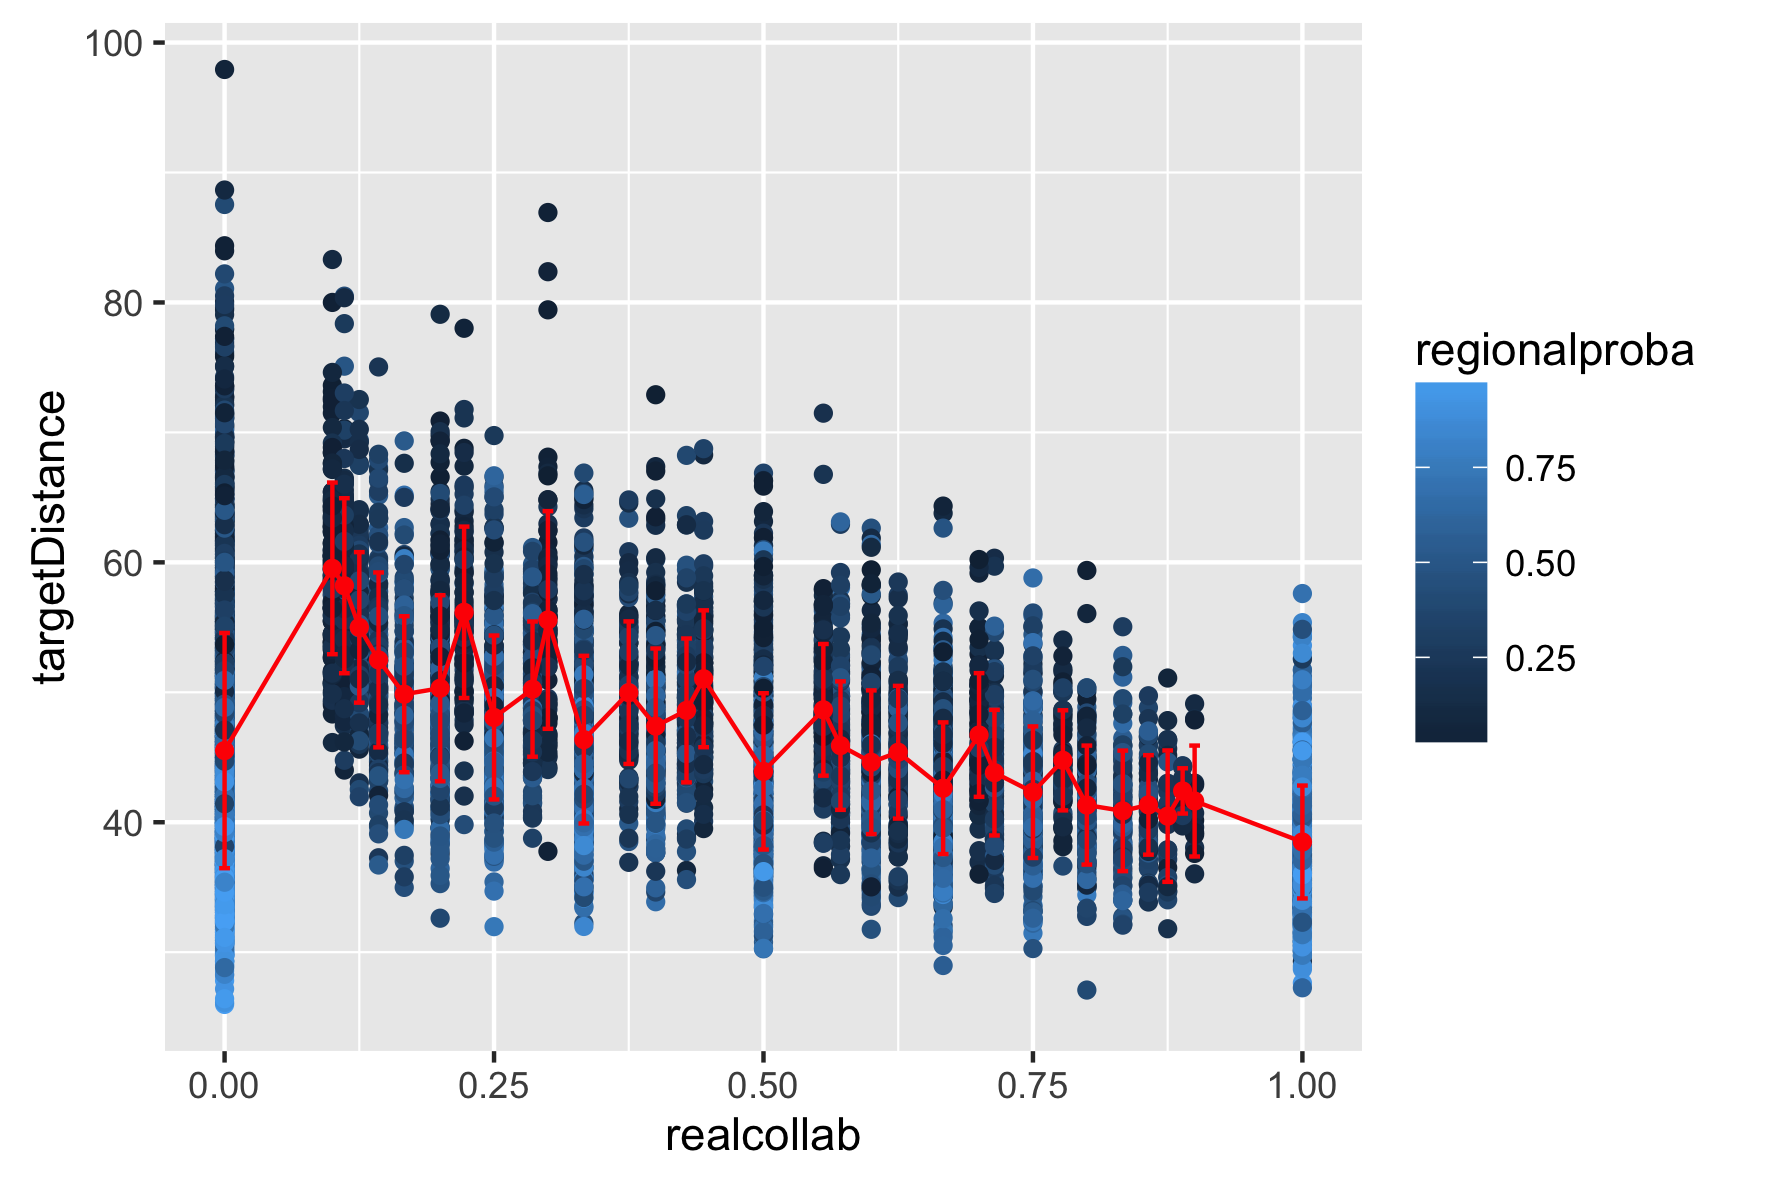
\includegraphics[width=0.49\linewidth]{Figures/Lutecia/collab-distance_colorregional.png}
	%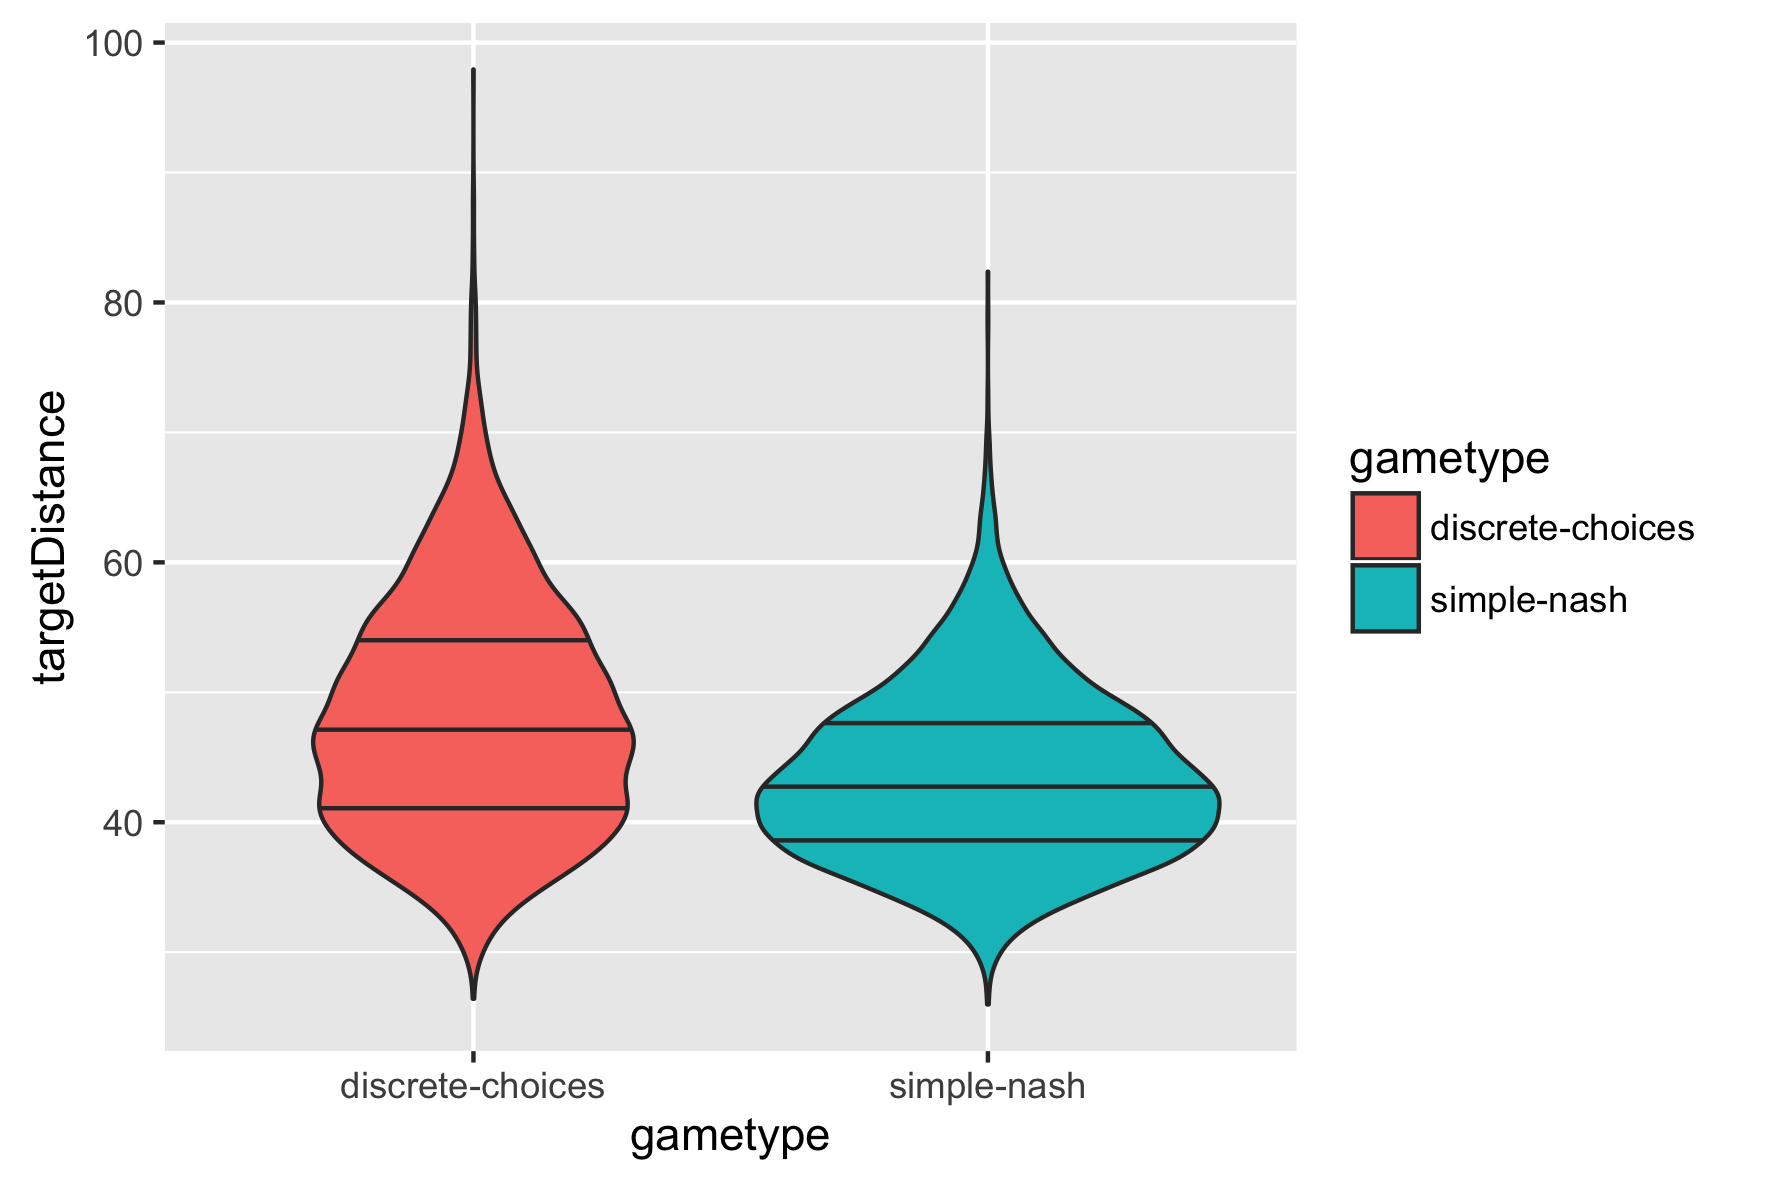
\includegraphics[width=0.49\linewidth]{Figures/Lutecia/distanceviolin_gametype.png}
	%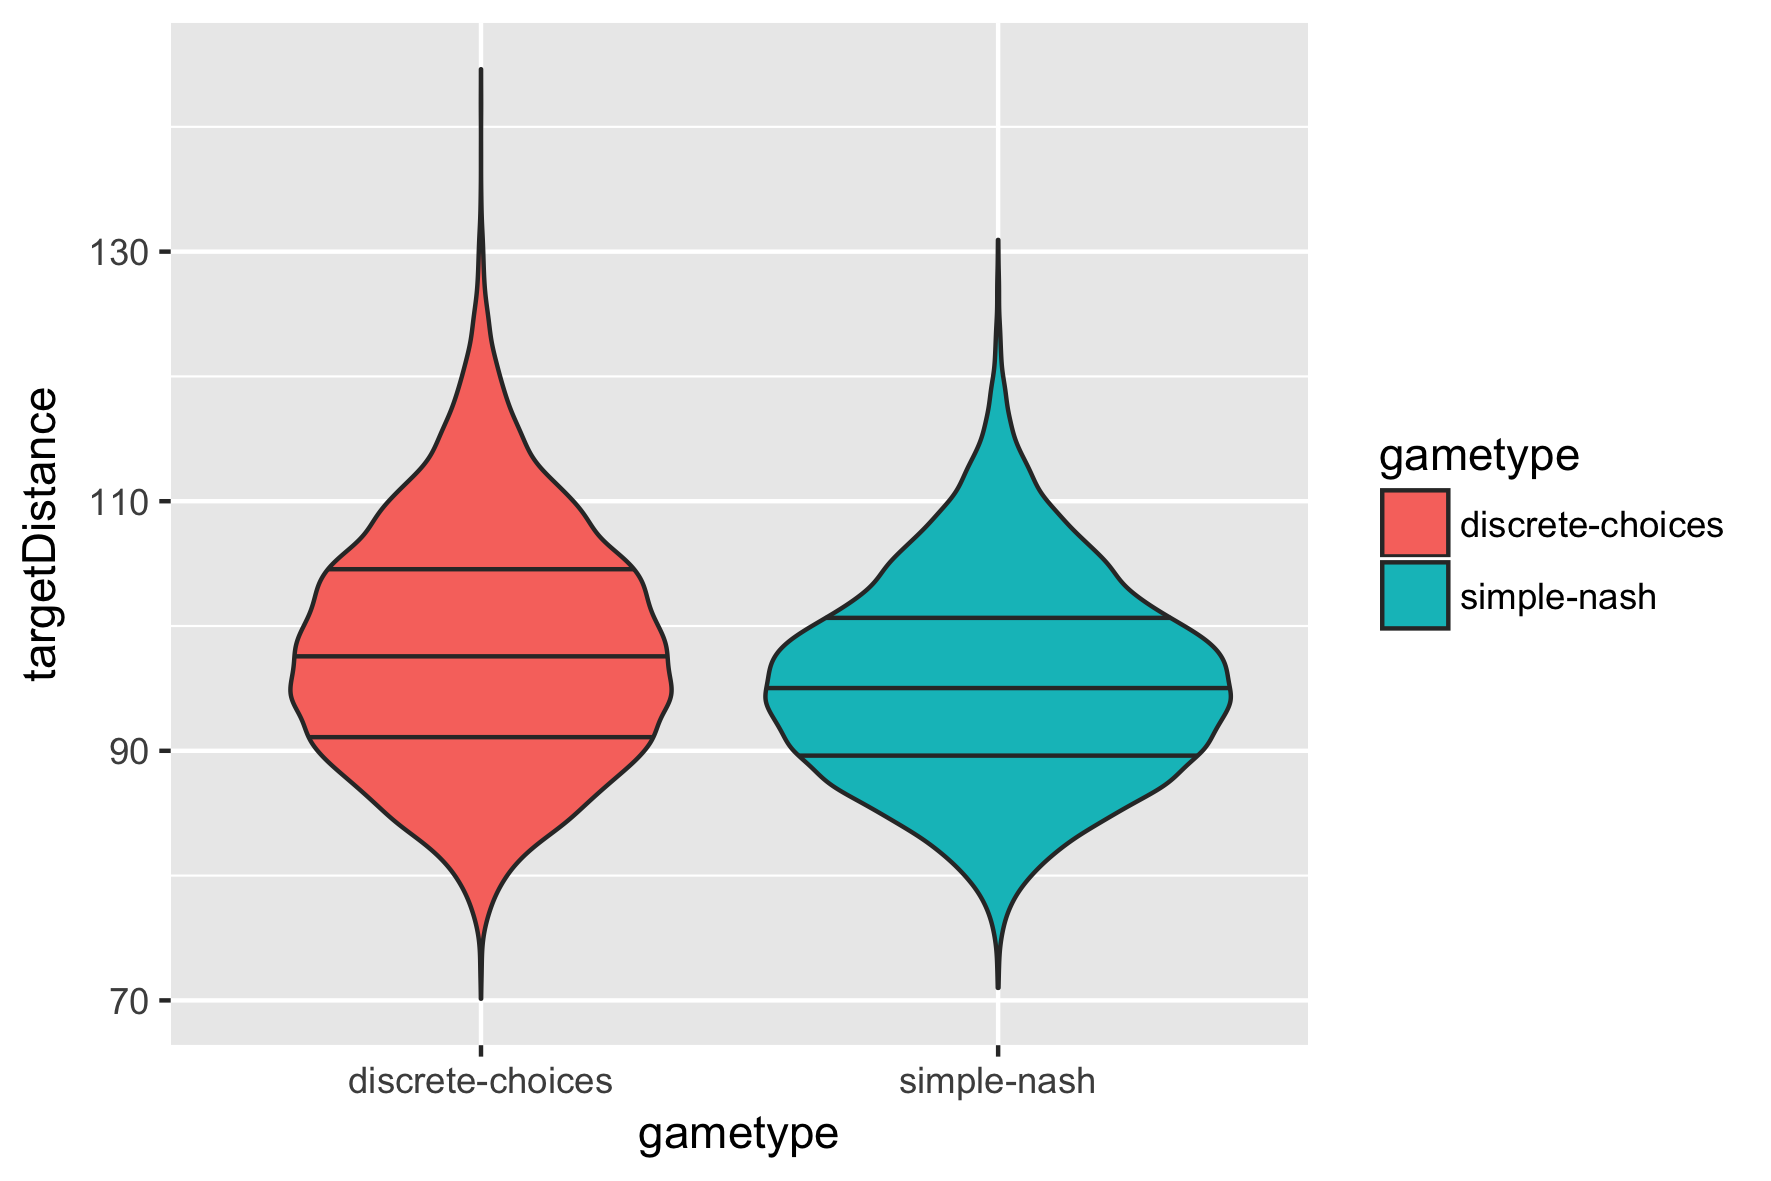
\includegraphics[width=0.49\linewidth]{Figures/Lutecia/distanceviolin_gametype_real.png}
	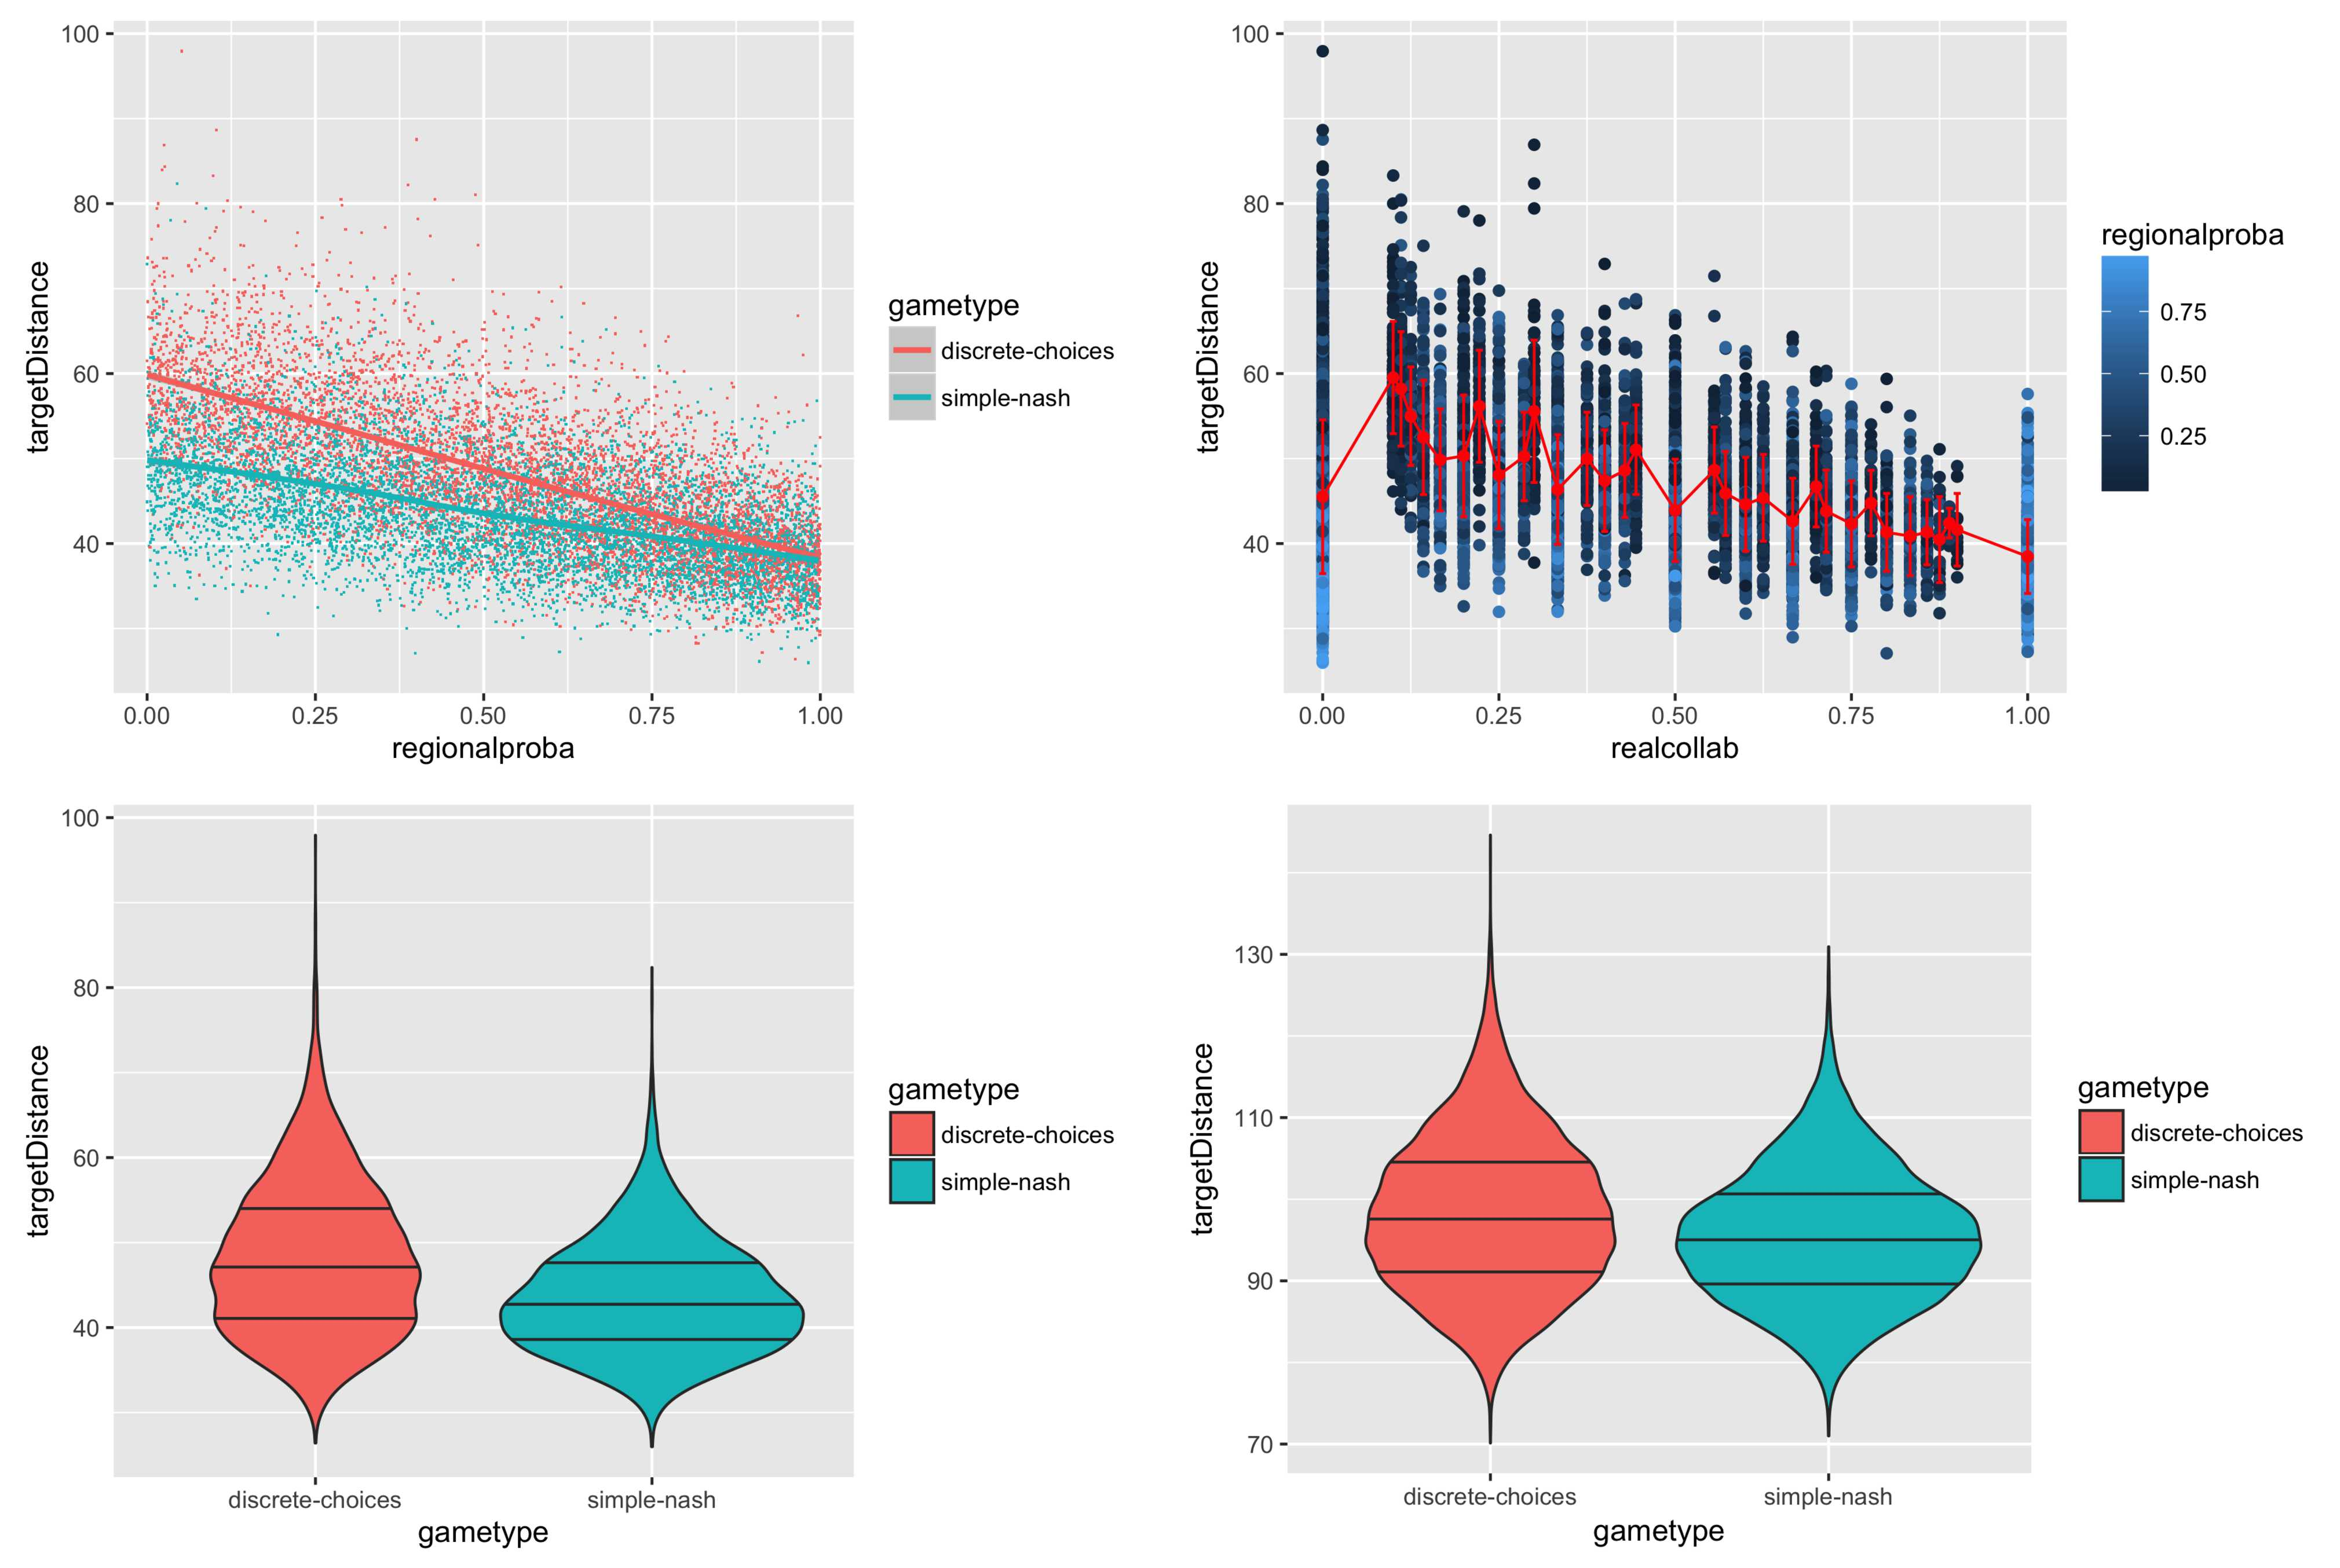
\includegraphics[width=\linewidth]{Figures/Final/7-3-3-fig-lutecia-calib.jpg}
	\caption[Calibration of the Lutecia model][Calibration du modèle Lutecia]{\textbf{Model calibration with fixed land use.} We take $\alpha = 0$ to make only network evolve, and sample the governance parameters space. (\textit{Top Left}) Distance $d_A$ to the target network (\texttt{targetDistance}), in the case of the real network, as a function of the regional decision probability $\xi$ (\texttt{regionalproba}), for the two types of games (colour). (\textit{Top Right}) Distance $d_A$ as a function of the observed collaboration probability (\texttt{realcollab}); the red curve gives the averages with standard errors. (\textit{Bottom Left}) Statistical distribution of distance as a function of the type of game, in the case of the real network; (\textit{Top Right}) in the case of the planned network. The difference between the types of games is larger in the case of the real network in comparison to the planned network.\label{fig:lutecia:calib}}{\textbf{Calibration du modèle à usage du sol fixé.} On prend $\alpha = 0$ pour ne faire évoluer que le réseau, et échantillonnons l'espace des paramètres de gouvernance. (\textit{Haut Gauche}) Distance $d_A$ au réseau cible (\texttt{targetDistance}), dans le cas du réseau réel, en fonction de la probabilité de décision régionale $\xi$ (\texttt{regionalproba}), pour les deux types de jeu (couleur). (\textit{Haut Droite}) Distance $d_A$ en fonction de la probabilité de collaboration observée (\texttt{realcollab}) ; la courbe rouge donne les moyennes avec les barres d'erreur. (\textit{Bas Gauche}) Distribution statistique de la distance en fonction du type de jeu, dans le cas du réseau réel ; (\textit{Bas Droite}) dans le cas du réseau planifié. La différence entre les types de jeux est plus grande dans le cas du réseau réel en comparaison au réseau planifié.\label{fig:lutecia:calib}}
\end{figure}
%%%%%%%%%%%%%%%


\bpar{
We thus draw from this experiment the following conclusions, to be naturally taken with caution.
\begin{itemize}
	\item A competition between actors is less probables than an egoistic behavior in the case of local decisions, since the discrete choices game give better performances than the Nash for low values of $\xi$.
	\item Collaboration compromises correspond to less probable networks than situations with full collaboration or with no collaboration.
\end{itemize}
}{
Nous tirons donc de cette expérience les conclusions suivantes, à prendre bien sûr avec prudence.
\begin{itemize}
	\item Une compétition entre les acteurs est moins probable qu'un comportement égoïste dans le cas de décisions locales, puisque le jeu par choix discrets donne de meilleures performances que le Nash pour les faibles valeurs de $\xi$.
	\item Les compromis de collaboration forment des réseaux moins probables que les situations avec pleine collaboration ou avec aucune collaboration.
\end{itemize}
}


\bpar{
These conclusions can be put into perspective with the increased competition within the Delta revealed by~\cite{xu2005city}. Thus, this application of the model allows to indirectly infer governance processes.
}{
Ces conclusions peuvent être mises en perspective avec la compétition accrue au sein du Delta révélée par~\cite{xu2005city}. Ainsi, cette application du modèle permet d'inférer indirectement des processus de gouvernance.  
}





\subsubsection{Discussion}{Discussion}


\bpar{
Although the model must still be more deeply explored and for all its modules, some possible developments are worth of interest.
}{
Bien que le modèle doit encore être exploré plus en profondeur et pour l'ensemble de ses modules, certains développements possibles peuvent retenir notre attention.
}


\paragraph{Endogenous level of decision}{Niveau de décision endogène}


\bpar{
One relevant extension would be the study of the emergence of larger administrative zones by aggregation, i.e. the emergence of new levels of governance in polycentric metropolitan areas. The example of the \emph{M{\'e}tropole du Grand Paris} is a good illustration for it when considering it in a simplified way, since it is positioned between local collectivities and the Region but also the State~\cite{gilli2009paris}. An extension of the model with rules to merge entities is a potential direction to study this question.
}{
Une extension pertinente serait l'étude de l'émergence de zones administratives par agrégation, c'est-à-dire l'émergence de nouveaux niveaux de gouvernance dans une région métropolitaine polycentrique. L'exemple de la Métropole du Grand Paris en est une bonne illustration en la considérant de manière simplifiée, puisqu'elle se situe entre les collectivités locales et la région ainsi que l'État~\cite{gilli2009paris}. Une extension du modèle avec des règles de fusion des entités est une direction potentielle pour étudier cette question.
}


\paragraph{Competition for an external ressource}{Compétition pour une ressource externe}


\bpar{
The influence of external territories or of externalities on the evolution of a MCR is an open question. In the case of a common resource, localized within the spatial extent of the MCR, competition or collaboration dynamics can emerge between actors for its exploitation. This model is a solution to study this situation in a stylized way, and thus realize a controlled experiment on co-evolution dynamics, which would allow to answer more general questions concerning the role of territorial isolation in co-evolution processes.
}{
L'influence des territoires extérieurs ou des externalités sur l'évolution d'une MCR est une question ouverte. Dans le cas d'une ressource commune, localisée dans l'emprise de la MCR, des dynamiques de compétition ou de collaboration peuvent s'instituer entre acteurs pour son exploitation. Ce modèle est une solution pour étudier cette situation de manière stylisée, et réaliser ainsi une expérience contrôlée sur les dynamiques de co-évolution, qui permettrait de répondre à des questions plus générales quant au rôle de l'isolation territoriale dans les processus de co-évolution.
}



\stars



\bpar{
We have thus build the first bricks of models aiming at a more complex integration of co-evolution processes, by developing the Lutecia model which was then validated in a preliminary way and which potentialities have been demonstrated by the application to the case study of Pearl River Delta.
}{
Nous avons ainsi posé les premières briques de modèles visant à une intégration plus complexe des processus de co-évolution, en développant le modèle Lutecia qui a ensuite été validé de manière préliminaire et dont les potentialités ont été démontrées par l'application au cas d'étude du Delta de la Rivière des Perles.
}







\stars




